\documentclass[12pt,
               phd,
               doublespacing
               ]{ncsuthesis}

\usepackage{longtable}
\usepackage{booktabs}
\usepackage{makecell}
\usepackage{multirow}
\usepackage{siunitx}
\usepackage{tabularx}
\usepackage{ragged2e}
\usepackage{rotating}
\usepackage{graphicx}
\usepackage{pdflscape}
\usepackage{array}
\usepackage{threeparttable}
\usepackage{amsmath}
\usepackage{textcomp}
\usepackage{xcolor}
\usepackage{lipsum}
\usepackage{glossaries}


\usepackage{tikz}
\usetikzlibrary{positioning}
\usetikzlibrary{fit}
\usetikzlibrary{shadows}


\usepackage[backend=biber]{biblatex}
\usepackage{float}
\usepackage[inkscapelatex=false]{svg}


\newacronym{pra}{PRA}{Probabilistic Risk Assessment}
\newacronym{mcs}{MCS}{Minimal Cut Sets}
\newacronym{mocus}{MOCUS}{Method of Obtaining Cut Sets}
\newacronym{bdd}{BDD}{Binary Decision Diagram}
\newacronym{obdd}{OBDD}{Ordered BDD}
\newacronym{lbdd}{L-BDD}{Labelled-BDD}
\newacronym{hpc}{HPC}{High Performance Computing}
\newacronym{saphire}{SAPHIRE}{Systems Analysis Programs for Hands-on Integrated Reliability Evaluations}
\newacronym{hra}{HRA}{Human Reliability Analysis}
\newacronym{qras}{QRAS}{the Quantitative Risk Assessment System}
\newacronym{ftrex}{FTREX}{Fault Tree Reliability Evaluation eXpert}
\newacronym{hcla}{HCLA}{Hybrid Causal Logic Analyzer}
\newacronym{kirap}{KIRAP}{}
\newacronym{ducg}{DUCG}{Dynamic Uncertain Causality Graphs}
\newacronym{ft}{FT}{fault tree}
\newacronym{et}{ET}{event tree}


\dispositionformat{\bfseries}

\headingformat{\large\MakeUppercase}

\frenchspacing

\include{optional}

\chair{Dr. Mihai A. Diaconeasa}

\student{Hasibul Hossain}{Rasheeq}

\thesistitle{Design and Implementation of a Distributed Networked System for PRA Quantification}

\newcommand{\uv}[1]{\ensuremath{\mathbf{\hat{#1}}}}
\newcommand{\bo}{\ensuremath{\mathbf{\Omega}}}
\newcommand{\eref}[1]{Eq.~\ref{#1}}
\newcommand{\fref}[1]{Fig.~\ref{#1}}
\newcommand{\tref}[1]{Table~\ref{#1}}
\addbibresource{bibliography.bib}
\begin{document}
\frontmatter
\begin{abstract}
Probabilistic Risk Assessment (PRA) is essential for risk-informed decision-making in industries such as nuclear, aerospace, oil and gas, chemical processing plants etc. However, the software tools used to analyze PRA models such as event trees, fault trees, and other risk models are often tied to specific operating systems and are hard to scale across different computing resources. This research work presents a domain specific distributed networked system that enables high throughput PRA quantification as a service. It provides a uniform, solver agnostic interface that brings multiple PRA engines together behind a single API gateway. The gateway isolates users from tool and operating system constraints and runs analyses on CPUs and GPUs across distributed memory and on-premise cluster. The research contributions can be divided into three parts. First, it provides a deployable microservice that runs PRA jobs asynchronously for multiple users and supports large volumes of jobs. It uses open source container orchestration to automate deployment, scaling, and routine management. Second, it includes an interoperability layer for PRA solvers that uses a common job specification and converts user submitted models to the supported solver formats automatically. Third, it introduces a three-step preprocessing, processing, and postprocessing pipeline. A case study of MHTGR models using the system shows that the pipeline speeds up analyses of large models while still producing reliable quantification results. The platform also provides controlled environments with role based access for regulated and proprietary data. For the nuclear engineering community, the system enables repeatable, high volume PRA quantification that are easier to run, compare, and share. 
%It also provides a software foundation that can add future solvers without disrupting existing analysis practices.
\end{abstract}

\thesistableofcontents
\thesislistoftables
\thesislistoffigures

\mainmatter
\chapter{Introduction}
\label{chap:introduction}

\section{Background and Motivation}

Probabilistic Risk Assessment (PRA) is a structured, model based approach used to understand risk in complex engineered systems such as nuclear power plants. In practice, PRA (1) identifies possible initiating events and failure scenarios, (2) estimates how likely those scenarios are to occur (e.g., frequencies or probabilities), (3) evaluates their potential consequences, and (4) explicitly represents and propagates the uncertainties in the underlying models and data. By linking plant systems, operator actions, and accident progressions through models such as event trees and fault trees, probabilistic risk assessment (PRA) generates quantitative risk metrics that characterize potential failure scenarios, the mechanisms by which they may occur, their estimated frequencies and consequences, and the confidence associated with those estimates.

PRA insights are usually combined with deterministic analyses, engineering judgment, and explicit safety margins to support risk-informed decision-making. This integration helps utilities and regulators prioritize attention and resources toward the most safety significant systems, components, and operational actions, while maintaining the conservative principles required in nuclear safety.

A central part of PRA is quantification: turning large logical models and reliability data into numerical results. Many commonly used quantification activities are computationally intensive, especially when performed repeatedly for configuration changes or model updates. Examples of such demanding tasks include computing (i) system failure probabilities from fault trees, (ii) event sequence frequencies from event trees, (iii) safety integrity level related metrics where applicable, (iv) common cause failure impacts, (v) importance measures used to identify risk significant components and operator actions, and (vi) the propagation of parameter uncertainty and (vii) sensitivity studies. These are not the only quantifications performed in PRA, but they represent a set of core calculations that frequently dominate runtime and are central to day-to-day risk studies.

The computational burden increases further as the scope of PRA expands to multi-hazard and multi-unit scenarios. External hazards, coupled dependencies, shared systems, and correlated failures can significantly increase the model size, producing very complex logic models.

For the nuclear energy sector, the ability to quantify these complex PRA models is not just a technical convenience, it is also linked to safety assurance and regulatory compliance. Plants must be able to perform thorough analyses, update risk models, support audits and reviews, and, deliver results on timelines that align with operational needs.

Despite the importance of these analyses, the current PRA software ecosystem remains difficult to access, difficult to integrate across platforms, and difficult to scale to the computational demands of complex PRA models. PRA tools are often inaccessible due to licensing issues and costs, and they are incompatible across workflows because the ecosystem is fragmented. This fragmentation is driven by several practical realities: nuclear plant data and models are often proprietary; tool developers have adopted different architectural and methodological philosophies (for example, differences in event tree linking versus fault tree linking approaches); and there is no standard data format that consistently represents PRA inputs, intermediate data structures, and results across tools. As a result, each platform tends to define its own data structures (often layered on top of general purpose formats such as XML, JSON etc.), and transferring a model from one tool to another typically requires tool specific knowledge. Conversions can be time consuming, error prone, and sometimes inherently lossy when data fields do not map properly. Operating system dependencies and vendor lock-in incentives further reinforce these issues.

Performance and scalability limitations compound the problem. Many existing tools are designed primarily for single user desktop workflows, offering serial execution or limited parallelism, often exposed through outdated GUIs or script oriented interfaces. For complex models, full quantification can take hours or even days, and practitioners may have limited visibility into whether a long running job is progressing normally or has stalled. When runs fail or appear stuck after extensive runtime, analysts may be forced to restart calculations, wasting time and compute resources. These constraints make it difficult to support time sensitive use cases (for example, near real-time evaluations during plant operation) and frequently encourage the use of truncation limits to keep calculations tractable. In practice, truncation thresholds are often selected based on experience and engineering conventions, but there is limited universal guidance, and the tradeoff between runtime and completeness can be difficult to manage transparently.

However, recent advances in open source containerization, message queueing, and microservices architectures create a clear opportunity to modernize PRA quantification workflows. A domain specific, distributed queueing and execution service can provide a unified API gateway that is operating system agnostic, supports automated deployments, and coordinates execution across modern heterogeneous hardware (GPUs, multi-core CPUs, FPGAs etc). Such a platform can also provide observability, traceability, and managerial control features that are important in regulated environments. The same design should support both cluster based deployments and a single node distributed memory based deployment, where each CPU core and available GPU can operate as an independent worker process with isolated resources (memory, compute allocation, and I/O), enabling distributed execution even without a multi machine cluster.

This work pursues that direction by designing and evaluating a distributed networked quantification platform for PRA. The study focuses on how such a system affects key operational and computational outcomes such as scalability, throughput, latency, and interoperability aiming to reduce analysis time, improve reliability and observability of long running quantifications, and lower integration barriers for PRA practitioners, tool developers, and organizations that must collaborate on complex risk models.

\section{Objectives}
This research work aims to accomplish the following objectives:
\begin{enumerate}
    \item Design a domain specific, operating system agnostic microservice that exposes a unified REST API gateway for PRA quantification and supports multi user, asynchronous submission.
    \item Define a common job specification and interoperability layer that decouple model submission from solver specific formats and interfaces.
    \item Integrate multiple PRA solvers by creating tool specific endpoints, demonstrating how both Windows and Linux based solvers can be supported.
    %\item Design and implement a priority-aware scheduling mechanism for a distributed queueing system that reduces latency for high-priority tasks (e.g., uncertainty quantification) while maintaining high throughput for mixed workloads under heavy load.
    \item Develop worker runtimes for CPUs and GPUs that scale across on-premise clusters or across distributed memory based deployments by treating each CPU core and each GPU on a node as an independent worker.
    \item Provide preprocessing, processing, and postprocessing workflows to enable distributed quantification of large models, including very large event trees.
    \item Leverage open source container orchestration to automate most deployment, scaling, and life cycle management tasks while preserving manual control where needed.
    \item Instrument the platform with standardized telemetry for latency, throughput, and error rates to support monitoring.
    \item Conduct a comprehensive evaluation that compares serialized, parallel, and distributed execution, quantifies speedup across models and calculation types, and characterizes scaling with the number of workers.
    \item Enforce role managed access and isolated execution to accommodate proprietary plant data and license restrictions.
    %assesses priority handling under mixed workloads,
    %and analyzes overheads for small, medium, and large models.
    \item Provide comprehensive documentation including implementation details, deployment configurations, experiment scripts, and functional and benchmark tests to enable reproducibility, guide users in deploying the system, and support integration of new solvers into the distributed platform.
\end{enumerate}

\section{Thesis Organization}
This thesis is structured as follows. Chapter 2 reviews the current PRA software landscape, identifies limitations in current workflows, and surveys related work in distributed computing for PRA. Building on this foundation, chapter 3 establishes the motivation for a distributed approach to PRA quantification and introduces the relevant distributed systems theory, architectural patterns, and design requirements. Chapter 4 then presents the overall system design, detailing its architecture, components, data flow, and key considerations for scalability and interoperability. The implementation of this design is described in chapter 5, covering the technology stack, task execution mechanisms, and deployment strategies. Chapter 6 presents the experimental methodology and results from a case study on MHTGR models and summarizes the key findings. These results are then discussed, including a comparison with a state-of-the-art tool supported by the NRC and an analysis of the distributed system's strengths and limitations. Finally, Chapter 7 concludes by summarizing the contributions and outlining directions for future work. Supplementary material, including source code, experiment scripts, and user documentation is provided in the Appendix.

%%\section{Problem Statement}
%%PRA practitioners lack a publicly available, locally deployable platform that scales quantification across heterogeneous resources while preserving tool interoperability, data governance, and reproducibility. In particular:
%%\begin{enumerate}
%%    \item Tool heterogeneity: PRA solvers use different model formats, assumptions, and execution interfaces, complicating interoperability and comparative studies.
%%    \item Limited scalability: Many tools prioritize serial execution or ad hoc parallelization and do not provide a distributed, multi tenant service for submitting and scheduling large batches of jobs.
%%    \item Operational constraints: Operating system dependencies and desktop centric deployments hinder reproducible and portable execution across environments.
%%    \item Governance and licensing: Proprietary plant data and tool licenses necessitate on-premises, role managed execution with strict isolation and auditability.
%%    \item Workload management: Mixed workloads require priority aware scheduling to control latency and fair distribution of computational resources under load.
%%    \item Resource heterogeneity: Practical deployments must utilize CPUs and GPUs efficiently, including single node scenarios where each core and the integrated GPU serve as independent workers.
%%   \item Distributed model decomposition and aggregation: Users need the capability to partition large PRA models during preprocessing, execute the partitions concurrently across distributed workers, and deterministically aggregate the partial results during postprocessing to fully exploit the scalability of the distributed system.
%%\end{enumerate}
%%The research problem is to design, implement, and evaluate a distributed queueing system that addresses these constraints for PRA quantification without relying on external, closed infrastructures, and without forcing analysts to rework existing models or tools.
\chapter{Literature Review}
\label{chap:literature-review}

\section{Review Process}
\label{sec:lr-pra-tools-related}

This chapter reviews contemporary software tools used for probabilistic risk assessment (PRA). The focus is on tools that are currently available and in active use (or at least still distributed and usable today). Legacy or discontinued tools are not reviewed in detail, except where brief historical context is helpful.

The main comparison is summarized in the feature matrix in Table~\ref{tab:pra_tools_overview}. To keep the review consistent and to avoid tool specific descriptions, each software is characterized using the same set of questions. These questions cover the practical, technical and computational aspects of these tools:

\begin{enumerate}
  \item \textbf{Interface:} Does the tool provide a web-based platform that can be accessed through any device? If not, then is it primarily command line based, graphical interface based, or does it support both? Can the CLI be used for batch runs?

  \item \textbf{OS dependency:} Which operating system(s) does the tool depend on? Windows, Linux, macOS, a combination of these 3 or all of them?

  \item \textbf{Licensing:} Is the tool open source, closed source, or free-to-use? Is a license explicitly stated? If a paid license is required, what are the constraints (single user, single machine etc.)?

  \item \textbf{Interoperability:} In what format is the model provided to the tool, and in what format are results produced (e.g., OpenPSA XML, JSInp)? Can the tool import and export models or results for interoperability with other tools?

  \item \textbf{Execution model:} Can the tool execute the tasks in a parallelized way (multi-core), or does it support only serial runs? Does it support distributed, networked execution across multiple machines?

  \item \textbf{Robustness:} If a run fails, becomes stuck, or encounters numerical/modeling errors, does the tool provide error messages and logs that can be used to diagnose the problem?
\end{enumerate}

In addition to reporting tool features, the discussion highlights where capabilities are mature and where gaps remain, especially regarding scalability and interoperability.

\section{Current PRA Tools}
\label{sec:lr-current-pra-tools}

The development of PRA software has progressed through distinct generations, from mainframe based cut set enumerators to contemporary GPU accelerated and decision diagram based solvers.

SAPHIRE \cite{saphire_8, saphire_809} is a long standing PRA suite developed for regulatory work. It is a Windows based desktop application with a GUI that supports graphical fault tree and event tree editing. Historically, it is not a web-based platform. However, recent work describes an extracted solver engine that can run on Linux as well, referred to as SAPHSOLVE \cite{diagnostics_strategies_saphire, refine_saphire_engine, enhancing_saphire_engine}, and explores cloud based solving to improve access to compute resources \cite{advancing_saphire}. SAPHIRE is closed source and its distribution is controlled through agreements and restricted access. SAPHIRE~8 is commonly associated with MAR-D style flat file databases for model and results storage, while SAPHSOLVE uses JSON based inputs/outputs to represent large model logic and solver results. The supported quantifications include MCS generation and probability and frequency quantification, importance measures, uncertainty analysis, and risk metrics such as CDF and LERF. It also supports operational event assessment outputs such as CCDP. The core quantification approach is traditionally cut set based and uses standard approximations, such as min-cut upper bound and rare event approximation alongside Monte Carlo or Latin hypercube sampling for uncertainty. Execution is historically serial for the desktop workflow, while recent plans and prototypes discuss parallel and distributed execution concepts for the extracted solver.

Phoenix Architect \cite{phoenix_architect_v2} is an EPRI managed commercial toolset intended to support a broad PRA workflow, including internal and external event based calculations. It runs on Windows desktop environment with a GUI, while some engines can also be used in batch style workflows through configuration and command line execution options. It is proprietary commercial software with licensing restrictions. Documentation commonly highlights export control constraints and non-disclosure requirements. An educational version exists, but it typically enforces explicit model size limits. The toolset \cite{phoenix_architect_v2_appendices} uses several module specific file formats, for example \texttt{.CAF} for fault trees, \texttt{.ETA} for event trees, and \texttt{.RR} repositories/databases), and commonly exports cut set results (\texttt{.CUT}, \texttt{.RAW}) and report outputs to formats such as Excel or database files. Interoperability is a notable feature: Phoenix Architect is described as supporting exchange with formats such as MAR-D, OpenPSA, and SETS. Quantification capabilities include linked ETs with FTs quantification for CDF and LERF, MCS generation, importance measures (FV/RAW/RRW/Birnbaum), uncertainty analysis, scenario based conditional risk calculations (such as CCDP), and external hazard risk studies (e.g., seismic and fire). Algorithmically, it supports both decision diagram based exact probability computation and cut set based calculations, and uses Monte Carlo or Latin hypercube sampling for uncertainty propagation. In execution mode, it supports both serial and parallel runs, and documentation also mentions remote quantification options where jobs can be executed on separate machines.

CAFTA \cite{cafta_1987, cafta_1989, cafta_10, phoenix_architect_v2_appendices}  is a commercial Windows desktop application for fault tree and event tree modeling and quantification. It is GUI driven and focuses on interactive model building, data management, and reporting. CAFTA is proprietary and typically licensed, with multiple license tiers, for example, professional, educational, and demo versions. CAFTA uses native formats such as \texttt{.CAF} (fault trees) and \texttt{.ETA} (event trees), and commonly stores supporting data in repository/database files (e.g., \texttt{.RR}). Outputs include cut set files (\texttt{.CUT}, \texttt{.RAW}) and report exports (Excel/text). CAFTA supports common PRA quantifications such as MCS generation, top event probability, importance measures, and uncertainty analysis. The cut set generation is typically ZBDD based and cut set probability approximations like MCUB and REA are used for probability calculation, while exact probability calculation is available through BDD based modules. In terms of execution, CAFTA’s core cut set engine is commonly described as serial. Higher performance and parallel execution are often achieved by integrating external solver engines (such as FTREX) rather than relying only on the native engine. For collaboration, CAFTA offers a repository feature that supports multi user teamwork through LAN/server based check in/check out and version history.

FTREX \cite{ftrex_2008, ftrex_2009} is a standalone fault tree solver engine that is commonly used as a backend quantification tool inside larger PRA environments \cite{ftrex_2020}. It is a Windows based application with a CLI interface and is typically commercially licensed with machine bound restrictions. It accepts multiple input formats used in industry workflows, for example, FTAP \texttt{.FTP} and KIRAP \texttt{.KIR}) and can output cut sets in formats such as \texttt{.RAW}, \texttt{.CUT}, and generic text. It can also export logic in formats used for exchange with other ecosystems (e.g., MAR-D files). FTREX supports minimal cut set generation, top event probability computation using cut set approximations (MCUB and REA), importance measures, and multi top quantification workflows that are used for quantifying CDF and LERF. It also supports prevention and path set style calculations for applications such as vital area identification. Algorithmically, FTREX relies on ZBDD structures for efficient MCS generation, and newer versions include BDD based exact probability computation. It also includes delete term approximation options for handling negations in specific settings. FTREX supports parallel execution on a single machine by splitting the problem (for example, by initiators or initiator groups) and solving parts concurrently using a wrapper workflow; this is shared memory parallelism rather than multi node cluster computing.

ZEBRA \cite{zebra_2024} is a recent solver engine focused on accurate quantification of noncoherent fault trees. Public descriptions present it primarily as a computation engine (with no dedicated GUI explicitly described), and the operating system and licensing model are not always clearly stated in publicly available materials. ZEBRA accepts fault tree logic and produces minimal cut sets for coherent models as well as prime implicants (PIs) for noncoherent models. these outputs enable accurate risk metric calculations (e.g., CDF estimation) compared to approaches that rely only on delete term approximations. The core method is based on zero suppressed ternary decision diagrams (ZTDD), which represent positive, negated, and "don’t care" states directly and can therefore encode noncoherent logic. ZEBRA supports both serial and multi thread parallel execution strategies \cite{zebra_2025}. Examples include initiator group partitioning and breadth first parallel solving of gates with reuse of previously computed results across worker threads.

XFTA \cite{xfta_2011, xfta_2020} is a cross platform fault tree calculation engine distributed as freeware (free to use) but not open source. It runs on Windows, Linux, and macOS (64 bit), and it is primarily a CLI tool, with a separate GUI frontend available in some workflows. The software distribution includes explicit restrictions against reverse engineering. XFTA supports OpenPSA XML inputs and also supports a textual, human readable modeling format called S2ML+SBE). Results are typically written as TSV files to support post-processing in spreadsheets and scripts. XFTA supports MCS extraction and ranking, top event probability calculations (including time dependent analysis), a broad set of importance measures, Monte Carlo based sensitivity analysis, and safety integrity level (SIL) metrics such as PFD and PFH. Its methods include a branch-and-test algorithm (SAT inspired) for direct MCS extraction, BDD based exact probability computation, ZBDD representations for compact MCS set handling, and standard cut set probability approximations (REA/MCUB/PUB). XFTA is primarily documented as a serial engine. Performance improvements are mainly achieved through data structure choices, caching, and careful compilation rather than explicit multi threading or distributed execution.

RiskSpectrum \cite{riskspectrum_website, riskspectrum_1990} is a commercial Windows based PRA suite with GUI editors for fault trees and event trees, and modules that support both detailed model development and operational risk monitoring. Its primary modeling environment is desktop based, while the RiskWatcher module uses a client-server architecture for monitoring and viewing risk results in an operational setting (network enabled access to results) \cite{riskspectrum_2010}. RiskSpectrum is proprietary and commercially licensed. Models are typically built using the internal editors, and the tool supports data import and integration workflows, for example, importing plant databases and linking with external fire modeling pipelines. Outputs include minimal cut sets, CDF and LERF results, importance measures and uncertainty results. Scripting support is also described for batch updates and model maintenance. The core quantification is traditionally cut set based, and a BDD solver is available to support exact probability calculations for complex logic. Public sources emphasize the ability to handle very large models, but they often provide limited detail on how much multi core parallelism is used for a single quantification run.

RISKMAN \cite{riskman_2009} is a proprietary commercial software that has a GUI and is commonly presented as part of an industry supported ecosystem, including interfaces to other tools. RISKMAN is described as providing built-in interfaces to other fault tree tools including CAFTA, FTREX, and SAPHIRE to support integrated workflows. Its quantifications emphasize event sequence evaluation, importance measures (including FV/RAW/RRW/Birnbaum and additional fractional measures), and uncertainty analysis using something called "Big Loop" Monte Carlo. It also includes hazard related analysis modules such as fragility based workflows and scenario screening (e.g., seismic and fire screening). Publicly available documentation typically provides limited detail on parallel or distributed execution.

ASTRA \cite{astra_1999, astra_2008, astra_3, astra_3x} is a Windows based GUI tool developed as an institutional fault tree analysis package. It supports importing and exporting the OpenPSA model exchange format and also uses native project and model file formats for storage. Public documentation describes a wide range of quantifications, including unavailability and unreliability analysis (including time dependent evaluation), failure and repair frequency calculations (including PFH measures), expected number of failures over an interval, importance measures, determination of significant minimal cut sets, and uncertainty analysis \cite{astra_2010, astra_2012}. ASTRA is decision diagram based: it uses BDD solving for standard cases, labelled BDD techniques for noncoherent logic, and truncation based methods (e.g., truncated ZBDD and decomposition plus truncation) when full exact representations become too large. Monte Carlo simulation is used for uncertainty propagation. Execution is described mainly as serial.

RiskA is a Windows based PRA tool developed in C\# and \texttt{.NET} ecosystem \cite{riska_2015, riska_5}. It is primarily a desktop GUI based application, and it also has a web-based collaborative modeling feature for fault tree models. Public sources do not clearly state whether RiskA is released under an open source license or a commercial license. For interoperability, RiskA supports a native XML based format and is described as importing OpenPSA MEF XML \cite{riska_2013}, as well as importing model files originating from other industry tools \cite{riska_2016}. Results are commonly exported to Excel and text formats. RiskA supports both qualitative and quantitative fault tree analysis, including MCS generation and prime implicants, top event probability, importance measures (FV/RAW/RRW/Birnbaum), uncertainty and sensitivity analyses, and supporting workflows such as FMEA style reporting. Its core computational method is based on ZBDD \cite{riska_algorithm}, and Monte Carlo simulation is used for uncertainty propagation. The literature does not mention anything about multi threaded or distributed quantification support.

DeRisk \cite{derisk_2018} is a research oriented tool based on Dynamic Uncertain Causality Graphs (DUCG) \cite{ducg_2012}. It is described as a desktop tool with both GUI and CLI interaction modes, and it is implemented in a C\# ecosystem. The licensing model is not clearly specified in the reviewed sources. DeRisk supports classical fault tree quantification including qualitative MCS generation (including disjoint MCSs) and quantitative top event probability, and it supports a broad set of importance measures. A key feature is support for Dynamic Fault Tree behavior through sequential and dependency gates such as PAND, FDEP, SEQ, and SPARE. The working principle described in the literature relies on mapping and probabilistic reasoning within the DUCG representation to capture sequential dependencies without a full state space explosion. Execution is typically described as serial.

\textbf{Hybrid Causal Logic toolset (Trilith, IRIS, and HCLA):}
The Hybrid Causal Logic (HCL) family extends classical FT and ET approaches by integrating event sequence diagrams, fault trees, and Bayesian belief network layers so that causal and socio-technical factors can influence hardware failure logic. In this toolset, IRIS \cite{iris_2007} is commonly described as a desktop GUI modeling environment (primarily Windows), Trilith \cite{trilith_2010} is a commercial Windows desktop application, and HCLA \cite{hcla_web} provides a solver engine that is available both as a cross platform CLI tool and through a web interface (OS agnostic for users). These tools are proprietary/research or commercial offerings rather than open source packages. Inputs are typically XML based model descriptions (often generated from the GUI tools), and outputs include quantitative risk metrics and importance rankings. Quantification capabilities include hybrid solving of ESDs, FTs and BBNs, uncertainty propagation (Monte Carlo, Latin hypercube, and quasi Monte Carlo), and time dependent results such as time-to-failure distributions and time dependent importance measures. The dynamic aspect is usually represented through time models and Bayesian conditioning of probabilities (probabilities change with causal context) rather than through explicit discrete event plant simulation. Public sources generally describe solver execution as serial; the web interface implies server side execution, but details of distributed multi node computation are not typically specified.

OpenPRA \cite{openpra_2023} is an open source web-based platform designed for collaborative PRA modeling and quantification. End users access it through a browser (GUI), while the quantification backend is implemented using containerization techniques, making it suitable for Linux based server environments and portable deployments. It is released under the MIT License. For interoperability, OpenPRA supports OpenPSA MEF XML and also uses JSON based schemas for frontend to backend communication and validation. Outputs can be produced in XML and JSON forms, including cut sets and quantitative results. It supports a broad set of standard PRA quantifications: MCS generation, exact and approximate probability quantification, importance measures, uncertainty analysis via Monte Carlo sampling, event sequence quantification, and CCF analysis. Algorithmically, it relies on engines that implement methods such as BDD and ZBDD, and supports MOCUS based cut set generation as well, and standard cut set approximations (MCUB and REA), alongside Monte Carlo solvers for uncertainty. OpenPRA is designed for distributed execution: it uses a queue based architecture (message broker and worker pool) to distribute jobs across multiple machines and supports concurrent execution of multiple quantifications.

\textbf{SCRAM and its modified versions: }
SCRAM \cite{rakhimov_scram_2022} is a free and open source PRA engine released under GPLv3. It is cross platform (Linux, Windows, macOS) and provides both a CLI interface for headless and batch workflows and a desktop GUI (Qt based) for visualization and interactive use. SCRAM supports OpenPSA MEF XML as its primary input format and produces XML reports. The GUI can export diagrams (e.g., SVG). Supported quantifications include fault tree and event tree quantification, MCS generation and prime implicants (for noncoherent trees), top event probability, importance measures, uncertainty analysis via Monte Carlo sampling, safety integrity level (SIL) metrics, and common cause failure (CCF) analysis using standard CCF models. Methods include MOCUS based cut set generation, BDD based exact probability calculations, ZBDD based set representations, and Monte Carlo sampling for uncertainty. The core solver is generally described as serial for a single quantification run.

SCRAM-cpp \cite{scramcpp_2026} is an enhanced C++ backend engine that builds on the SCRAM ecosystem and is designed for improved performance. It is operated as a CLI solver and is intended to be cross platform, with development and benchmarking often reported on Linux. It continues to use OpenPSA MEF XML as input and output format. A key contribution is explicit shared memory parallelization (e.g., with OpenMP) for computationally heavy tasks such as importance measures and uncertainty sampling, where multi core speedups are reported in benchmark studies. Design discussions also outline directions for distributed memory execution (e.g., MPI) to address problems that exceed single node memory limits, although this is often presented as a roadmap rather than a universally available production feature.

SCRAM++ \cite{scram++_2025} is described as a research platform that wraps multiple quantification algorithms into a unified workflow and selects between them depending on fault tree structure. It is designed to work with OpenPSA MEF inputs and produces standard quantitative outputs (probabilities and cut sets). Its main focus is algorithmic scalability and specialization for applications such as seismic PRA and fragility analysis. A distinguishing method is the use of compressed truth table style formulations to compute exact probabilities efficiently for certain structures such as gates with multiple occurring events, alongside more traditional BDD, ZBDD and MOCUS methods. Public descriptions emphasize serial performance improvements and hybrid method selection more than explicit parallel or distributed execution.

mcSCRAM \cite{arjun_mcscram} is a high performance Monte Carlo engine developed in the SCRAM ecosystem and designed to run efficiently on multi core CPUs and GPUs using SYCL based backend. It is a CLI tool and does not provide a dedicated web interface on its own. mcSCRAM is released under the AGPLv3 license, which has important implications for network deployment (source availability requirements when used as a service). It supports OpenPSA MEF inputs and produces probability estimates and statistical outputs consistent with the SCRAM style reporting approach. Unlike deterministic cut set or BDD solvers, mcSCRAM focuses on data parallel Monte Carlo: it compiles the model into a probabilistic circuit (a DAG representation of the logic), evaluates many Monte Carlo trials at once using bit-packed Boolean vectors, and uses counter based Philox random number generation to support massive parallel sampling without synchronization overhead. This design provides strong parallel performance on a single heterogeneous node (GPU and CPU). Public descriptions generally do not claim multi node distributed execution across a cluster, and the tool is described as being in an early/alpha stage.

\section{Existing Distributed Computing Approaches for PRA}
\label{sec:lr-parallel-distributed}

Across the reviewed tools, most PRA quantification still assumes a single machine execution model. In many commercial desktop environments, the default workflow is serial execution on a Windows workstation, with scalability achieved mainly through solver efficiency, approximation settings, or splitting the study into multiple independent runs. Parallelism is more common in (i) uncertainty analyses that require many repeated samples (e.g., SCRAM-cpp), (ii) batch evaluation of many sequences or many top events (e.g., Phoenix Architect, FTREX), and (iii) Monte Carlo simulation engines that can spread trials across CPU cores or GPU threads (e.g., mcSCRAM).

A smaller set of tools describe stronger forms of parallel execution. Some solver engines parallelize by partitioning a large model into smaller independent subproblems and solving them concurrently on a multi core machine (e.g., ZEBRA). Some open source engines explicitly parallelize internal loops for importance and uncertainty calculations using shared memory programming models (e.g., SCRAM-cpp). Monte Carlo based tools can achieve substantial speedups on GPUs (e.g., mcSCRAM), but they often focus on saturating a single heterogeneous node rather than scaling across multiple networked machines.

Distributed, networked execution where multiple worker machines are coordinated through a queue and a central scheduler is described much less often in public documentation. Among the reviewed tools, OpenPRA provides a clear end-to-end distributed design: it uses a message broker, a scalable worker pool, task decomposition, and operational fault handling mechanisms. A few commercial toolchains mention the ability to run quantification on remote machines (e.g., Phoenix Architect), but public sources typically provide fewer details about scheduling semantics and multi tenant queueing. Overall, the literature shows growing interest in web access and scalable computation, but openly specified distributed queueing infrastructures for heterogeneous PRA workloads are still uncommon.

\newcolumntype{L}[1]{>{\raggedright\arraybackslash\hsize=#1\hsize}X}
\newcolumntype{C}[1]{>{\centering\arraybackslash\hsize=#1\hsize}X}
\begin{landscape}
\begin{table}
\centering
\begin{threeparttable}
\scriptsize
\setlength{\tabcolsep}{4pt}
\caption{Feature overview of reviewed \acrshort{pra} tools.}
\label{tab:pra_tools_overview}

\begin{tabularx}{\textwidth}{@{} L{1.20} L{1.30} L{0.60} L{1.55} L{0.85} C{0.50} @{}}
\toprule
\textbf{Tool} &
\textbf{Platform/OS} &
\textbf{User} &
\textbf{Model Exchange Format} &
\textbf{License} &
\textbf{Processing Mode} \\
\midrule

\acrshort{saphire} &
Desktop/Windows &
Single &
MAR-D + JSInp &
Proprietary &
S \\

Phoenix Architect &
Desktop/Windows &
Multi\tnote{*} &
.CAF, .ETA, .RR, .CUT, .RAW + MAR-D + OpenPSA + SETS &
Commercial proprietary &
S/P/D\tnote{$\dagger$} \\

CAFTA &
Desktop/Windows &
Multi\tnote{*} &
.CAF, .ETA, .RR, .CUT, .RAW + SETS + FTAP &
Commercial proprietary &
S \\

\acrshort{ftrex} &
Desktop/Windows &
Single &
FTAP/.FTP + KIRAP/.KIR + .RAW, .CUT, .TXT + MAR-D &
Commercial proprietary &
P \\

ZEBRA &
Solver engine/OS n/s &
Single &
Unspecified &
Unspecified &
S/P \\

XFTA &
Desktop/Cross platform &
Single &
OpenPSA + S2ML+SBE + TSV &
Freeware proprietary &
S \\

RiskSpectrum &
Desktop/Windows + client-server &
Single\tnote{*} &
Unspecified &
Commercial proprietary &
S \\

RISKMAN &
Desktop/Windows &
Single &
CAFTA + FTREX + SAPHIRE &
Commercial proprietary &
S \\

ASTRA &
Desktop/Windows &
Single &
OpenPSA + .tfx, .adf &
Proprietary &
S \\

RiskA &
Desktop/Windows + client-server &
Multi &
XML + OpenPSA + CAFTA and RiskSpectrum formats + Rich text + Excel, text, Word &
Proprietary &
S \\

DeRisk &
Desktop/OS n/s &
Single &
Unspecified &
Proprietary &
S \\

Trilith &
Desktop/Windows &
Single &
XML export &
Commercial proprietary &
S \\

\acrshort{hcla} &
CLI/Cross platform + client-server &
Multi &
JSON &
Proprietary &
S \\

OpenPRA &
Client-server &
Multi &
OpenPSA + OpenPRA JSON &
MIT + GPLv3 &
D \\

SCRAM &
Desktop/Cross platform + Solver engine &
Single &
OpenPSA + SVG &
GPLv3 &
S \\

SCRAM-cpp &
Solver engine/Cross platform &
Single &
OpenPSA &
GPLv3 &
P \\

SCRAM++ &
Solver engine/Cross platform &
Single &
OpenPSA &
Proprietary &
S \\

mcSCRAM &
Solver engine/Cross platform &
Single &
OpenPSA &
AGPLv3 &
P \\

\bottomrule
\end{tabularx}

\begin{tablenotes}
  \item[*] ``Multi-user'' here refers to built-in support for team workflows (e.g., repositories or web access), not necessarily simultaneous editing of the same model without coordination.
  \item[$\dagger$] Phoenix Architect documentation mentions remote quantification options. Public sources do not describe full scheduling and fault tolerance semantics.
  \item[] Processing types: S = serial; P = parallel on a single machine (shared memory / GPU); D = distributed execution across multiple machines.
  \item[] n/s = not specified clearly in the reviewed public documentation.
\end{tablenotes}

\end{threeparttable}
\end{table}
\end{landscape}

\section{Limitations of Current PRA Tools}
\label{sec:lr-limitations}

The current software ecosystem of PRA exhibits recurring limitations that affect scalability, interoperability, and operational reliability. While some tools may partially address these problems, they are either proprietary or not yet fully developed. The following constraints are broadly observed across widely used desktop applications, command line quantifiers, and web-based platforms:

\begin{itemize}
  % \item External hazard models (e.g., fire, seismic) frequently contain tens of thousands of basic events, causing memory explosion and extended runtimes (hours or days) during minimal cut set (MCS) manipulation and decision diagram construction (BDD, ZBDD), particularly with noncoherent logic and deeply nested expansions.

  \item Operating system dependencies (often Windows centered) and local GUI runtimes hinder cross platform reproducibility and complicate execution in controlled compute environments (e.g., Linux based HPC clusters).

  \item Proprietary commercial tools impede external optimization for multi core, GPU, or cluster environments, limit independent verification, and restrict community driven improvements.
  
  % while open source alternatives often lack robust multi tenant service infrastructure and operational tooling expected in production settings.

  \item Most tools support only serial or single node parallel execution. Distributed submission interfaces are comparatively rare and, when present, are commonly tied to private script based schedulers rather than modern network accessible REST APIs with explicit resource governance.

  \item Current tools generally lack support for high volumes of simultaneous job requests with asynchronous execution, resulting in unpredictable turnaround times and inadequate priority handling for heterogeneous workloads (e.g., point estimate runs take less time compared to uncertainty quantification, importance measures and sensitivity studies).

  \item The absence of a unified platform that can host multiple solvers forces users to buy licenses for multiple solvers perform error prone conversions across different proprietary formats, impeding solver interoperability and making it difficult to compare results across quantification engines under controlled conditions.

  \item Sensitive nuclear plant data frequently necessitates on premise deployment, yet many tools lack built in identity and access management (IAM) integration and role based access controls (RBAC).

  % \item Per host licensing policies constrain scaling across on-premise cluster nodes, often limiting deployments to single node configurations, thereby reducing achievable throughput for large model batches.

  \item Most quantifiers lack native GPU support and heterogeneous resource orchestration, and any available thread level parallelism is rarely coordinated by a multi tenant scheduler.
  
  % This can lead to rapid saturation of available resources under concurrent usage.

  % \item Many quantifiers tightly couple parsing, compilation, quantification, and post processing in a single monolithic run, hindering scalable pre processing (e.g., parallel transformations of event tree sequences into individual fault trees), incremental compilation, and reuse of intermediate artifacts.

  % \item Standardized reporting of performance and service quality metrics (e.g., latency, throughput, queue wait time, solver utilization, error rates) is uncommon. In the absence of such metrics, it is difficult to set technical requirements for web-based quantification services under multi user demand or to diagnose capacity bottlenecks.

  \item When large runs fail, stall, or encounter memory errors, tools typically print error messages but often do not indicate which specific part of the model (e.g., a particular event sequence) caused the problem or where the run became stuck. Logs are usually limited to overall run status (success/failure) or generic error messages, which makes triage and root cause analysis difficult. In contrast, a distributed networked execution system can isolate failures to specific sub jobs (e.g., sequence level tasks), retain per task logs, and provide actionable diagnostics.
\end{itemize}

Collectively, these limitations highlight the critical need for automated and portable deployment options, standardized interfaces, and scalable execution strategies that maintain data governance while accelerating processing times for large, realistic PRA models. They also motivate PRA execution platforms that treat quantification as an observable service: one that can schedule work, isolate faults, retain structured logs, and provide reproducible execution records across heterogeneous solvers and workloads.

\section{Summary}
\label{sec:lr-summary}

The PRA software ecosystem spans legacy cut set enumerators, mature desktop suites, command line quantifiers, causal modeling platforms, and emerging web enabled services. Each category offers distinctive strengths in areas such as comprehensive modeling environments, advanced quantification algorithms, or improved accessibility. However, the literature and current practice reveal some persistent limitations. These include OS specific deployments, constrained parallelism, limited support for distributed and asynchronous execution, proprietary formats that inhibit solver interoperability, weak service level observability, and incomplete security features for on-premise deployments. In addition, robustness remains a practical operational gap: when large batch computations fail or hang, available tooling often provides only coarse error output that does not pinpoint the responsible model component (e.g., an individual event sequence), increasing the time and effort required for debugging and rerunning large studies.

Prior works demonstrate important algorithmic improvements (e.g., decision diagram techniques) and introduces web-based mechanisms for remote execution. Nonetheless, the literature lacks comprehensive descriptions of a fully specified, solver agnostic, publicly available queueing and execution system designed to support heterogeneous PRA workloads under multi user demand, with explicit capabilities for prioritization, resource governance, structured logging, and failure isolation. The scalability, interoperability, robustness, and governance challenges documented in this review motivate the development of a systematic, high performance distributed computational solution, which forms the focus of subsequent chapters.

\chapter{Distributed Networked Systems: Theory and Practice}
\label{chap:distributed-systems}

\section{Necessity of Distributed Computation for PRA}
\label{sec:necessity-ds-pra}
The computational demands of modern PRA quantification create a compelling case for distributed approaches. PRA models for complex nuclear facilities, particularly for advanced reactors, integrate large event trees with functional events linked to fault trees across multiple initiating hazards. This architecture leads to a combinatorial explosion, where hundreds of event sequences linked to tens of fault trees can produce millions of logic gates and thousands of distinct basic events. The prevalence of k-out-of-n gates, which must be expanded into combinations of AND and OR gates, further increases this complexity. Furthermore, these models frequently contain non-coherent structures due to success paths, requiring exact solutions to avoid overlooking hidden prime implicants with significant probabilities. The presence of common-cause failures, shared support systems, and hazard-induced correlations invalidates the assumption of event independence, necessitating more sophisticated and resource intensive quantification. Additionally, calculating importance measures, performing sensitivity analysis on hundreds of fault trees, and applying extensive post-processing rules to event sequences to account for recovery actions or physical constraints each demand significant computational resources. Therefore, distributed computation becomes necessary not only for performance but also for feasibility. With current PRA tools, which often run serially or only with limited parallelism, executing all of these analyses together can be impractical because they may not finish within reasonable time limits or fit within the memory of a single machine.

The heterogeneity of PRA workloads makes them particularly well suited for distributed computation. Different quantification tasks, such as point estimation, importance measure calculation, sensitivity analysis, and uncertainty analysis, impose different computational and memory requirements. A distributed system can map these heterogeneous workloads onto available hardware more effectively; for example, memory intensive cut set manipulation can be assigned to machines with large RAM, while Monte Carlo based uncertainty calculations can be distributed across many CPU cores or accelerators when such hardware is available. This flexibility allows the computational strategy to be adapted to the structure of the PRA task rather than forcing all calculations through the limitations of a single execution environment.

The analysis workflow surrounding large PRA models also benefits substantially from distributed computation. Importance measure calculations can be parallelized at the basic event level, with each event's metrics evaluated independently, while individual simulation runs in Monte Carlo based uncertainty analysis can be distributed across computational nodes. Likewise, large scale post-processing of event sequence results can be divided across workers when rules are applied independently. More broadly, an open source distributed system gives the end user control over how and where that computation is deployed. Depending on organizational requirements, the same framework can be run on a single node, on a secure on-premise cluster, or on approved cloud infrastructure. In this way, the objective is not to prescribe a single deployment model, but to give PRA practitioners the ability to use the computational resources available to them while retaining control over performance, security, and operational constraints.

\section{Definition and Characteristics of a Distributed Networked System}
\label{sec:ds-definition}
A distributed networked system is a collection of independent computing nodes connected through a network that collaborate to appear as a single computing system to end users. Unlike a monolithic application running on a single machine, distributed systems spread processes and resources across multiple computers, enabling capabilities that would be impossible for any single node to achieve alone. Distributed systems are characterized by several key attributes \cite{steen_distributed_2023}:
\begin{itemize}
    \item \textbf{Partial failure:} meaning the ability to continue functioning despite partial failures, where some components may fail while others remain operational.
    \item \textbf{Resource sharing:} enables multiple users or applications to access and utilize hardware, software, and data across the network.
    \item \textbf{Distribution transparency:} represents the ideal goal of hiding the distributed nature of the system, making it appear as a single unified entity, though in practice this abstraction is necessarily imperfect.
    \item \textbf{Dependability:} encompasses availability, reliability, safety, and maintainability, ensuring the system operates correctly even when faults occur.
    \item \textbf{Security:} protects against unauthorized access and malicious attacks across the distributed infrastructure.
    %\item \textbf{Openness:} allows systems to be built from standard, interoperable components that can communicate through well-defined interfaces.
\end{itemize}

When designing a distributed system, developers must address the "fallacies of distributed computing" i.e., common but false assumptions made in this domain \cite{wilson_eight_nodate}. Among these are the beliefs that the network is reliable, secure, and homogeneous; that latency is zero and bandwidth infinite; that topology does not change; and that there is only one administrator. Mature system design acknowledges these fallacies and builds mechanisms to handle them rather than pretending they don't exist. Correct designs implement strategies like timeouts, safe retries, failure containment etc. to manage these inevitable issues.

\section{Architectural Patterns}
\label{sec:architecture-patterns}
Distributed systems can be designed following several common architectural patterns, each suited for specific requirements \cite{steen_distributed_2023}:

\begin{itemize}
    \item \textbf{N-tier Client-Server Architecture:} In this pattern, \emph{clients} send requests to one or more \emph{servers}, and the servers process the requests and return responses, often by reading from or writing to a database. In practice, client--server systems are commonly implemented as an $N$-tier (layered) design, where requests flow through a \emph{reverse proxy} tier (routing, load balancing), then a \emph{business logic} tier (application services), and finally a \emph{database} tier. Each tier has a clear responsibility and communicates through well defined interfaces, which improves separation of concerns. The main trade-off is added complexity and overhead at the interfaces, and changes that span multiple tiers may require coordinated updates across their interfaces. Figure~\ref{fig:client-server} shows this $N$-tier flow: clients connect to a reverse proxy, which forwards requests to the business logic tier that interacts with the database layer before returning a response to the client.
    
    \begin{figure}[]
  \centering
  \includesvg[width=0.8\textwidth]{3-theory-and-practice/plots/client-server.svg}
  \caption{Example of an $N$-tier client-server architecture.}
  \label{fig:client-server}
\end{figure}

    \item \textbf{Service Oriented Architecture (SOA):} SOA builds applications from independent services that communicate over a network using standardized service contracts (a shared “language” such as HTTP/JSON). It is often used at the enterprise level to integrate separate systems so that different business domains can share information. SOA can improve reuse and integration, but as the number of services and shared contracts grows, the overall system can become more complex to manage. Figure~\ref{fig:service-oriented-architecture} shows a service oriented system where a client application composes functionality by calling multiple backend services through well defined interfaces.
    
    \begin{figure}[]
  \centering
  \includesvg[width=0.6\textwidth]{3-theory-and-practice/plots/service-oriented-architecture.svg}
  \caption{Example of a food delivery platform using a service oriented architecture.}
  \label{fig:service-oriented-architecture}
\end{figure}

    \item \textbf{Event Driven Architecture:} In event driven systems, components communicate by publishing and consuming \emph{events}. Producers publish events (e.g., \texttt{TransactionCompleted}) to an event broker or message channel, and consumers subscribe to the events they care about (e.g., receipt emails, analytics updates, loyalty points). This provides strong decoupling because producers do not need to know which consumers exist, and consumers can process events asynchronously (including catching up after downtime). This pattern is especially useful when many parts of a system must react to the same business activity and when keeping an event history is important. Figure~\ref{fig:event-driven-architecture} depicts an event broker that receives events from producers and delivers them to multiple subscribers, enabling asynchronous processing and loose coupling between services.
    
    \begin{figure}[]
  \centering
  \includesvg[width=0.8\textwidth]{3-theory-and-practice/plots/event-driven-architecture.svg}
  \caption{Example of an e-commerce website using an event driven architecture.}
  \label{fig:event-driven-architecture}
\end{figure}

    \item \textbf{Microservices Architecture:} Microservices decompose an application into small, independently deployable services, each responsible for a narrow business capability. Services typically communicate through APIs and can be developed, deployed, and scaled independently. Microservices can be viewed as a fine grained evolution of SOA, but they usually favor simpler protocols and more decentralized service ownership. The main trade-off is increased operational complexity such as deployment automation, monitoring, tracing, and managing distributed failures. Figure~\ref{fig:microservices} illustrates an e-commerce system split into multiple small services that the front end can call independently (e.g., catalog, checkout, payments).
    
    \begin{figure}[]
  \centering
  \includesvg[width=0.9\textwidth]{3-theory-and-practice/plots/microservices.svg}
  \caption{Example of an e-commerce website using a microservices architecture.}
  \label{fig:microservices}
\end{figure}

    \item \textbf{Peer-to-Peer (P2P) Architecture:} In a peer-to-peer system, nodes act as both clients and servers and share their own resources (storage, bandwidth, or compute) without relying on a central server. This pattern is common in file sharing systems and blockchain networks. P2P can improve resilience and avoid single points of failure, but it makes coordination, trust, and security more challenging. Figure~\ref{fig:peer-to-peer} shows a peer-to-peer network where nodes communicate directly with each other, forming a decentralized mesh for sharing data and work.
    
    \begin{figure}[]
  \centering
  \includesvg[width=0.8\textwidth]{3-theory-and-practice/plots/peer-to-peer.svg}
  \caption{Example of a blockchain network using a peer-to-peer architecture.}
  \label{fig:peer-to-peer}
\end{figure}
\end{itemize}

\section{Queueing Systems in Distributed Environments}
\label{sec:ds-queueing}
Queueing systems provide critical infrastructure for managing workload distribution and decoupling components in distributed systems. They act as buffers between producers and consumers of work, allowing systems to process variable loads of varying priorities and handle component failures gracefully.

Message brokers implement queueing patterns using either point-to-point messaging, where each message is consumed by exactly one consumer, or publish-subscribe messaging, where messages are broadcast to multiple interested consumers. These brokers provide durability by persisting messages to disk, ensuring that work isn't lost during system failures. They also enable load leveling by absorbing traffic spikes and distributing work to consumers at their optimal processing rate. The workflow for a typical message broker is shown in Fig. \ref{fig:message-broker}.

% \begin{figure}[h]
  \centering
  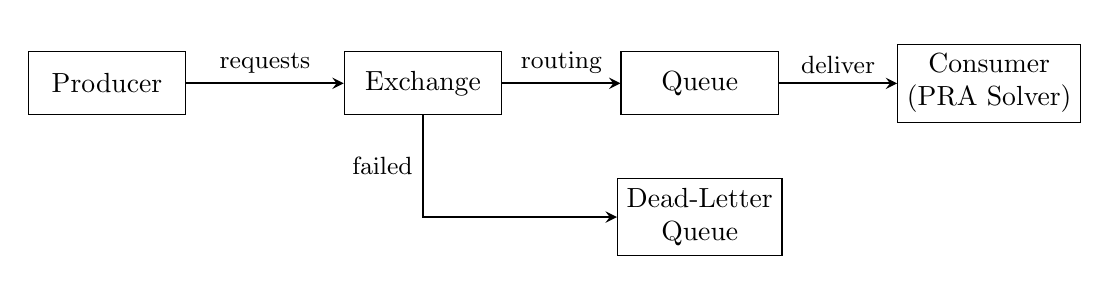
\begin{tikzpicture}[
      scale=0.7,
      >=stealth,
      box/.style={draw,rectangle,minimum width=2cm,
                  minimum height=0.8cm,align=center},
      msg/.style={->, thick},
      label/.style={font=\small,draw=none}
    ]
    
    % Message Broker components
    \node[box] (exchange) {Exchange};
    \node[box, right=1.5cm of exchange] (queue) {Queue};
    \node[box, below=0.8cm of queue] (dlq) {Dead-Letter\\Queue};
    
    % Fit node for RabbitMQ Message Broker
    \node[fit=(exchange)(queue)(dlq),
          draw, inner sep=0.3cm, dashed, 
          label={[yshift=0.3cm]\textbf{RabbitMQ}}] (broker) {};
    
    % Publisher and Consumer
    \node[box, left=2cm of exchange] (producer) {Producer};
    \node[box, right=1.5cm of queue] (consumer) {Consumer\\(PRA Solver)};
    
    % Draw connections
    \draw[msg] (producer) -- node[above,label]{requests} (exchange);
    \draw[msg] (exchange) -- node[above,label]{routing} (queue);
    \draw[msg] (queue) -- node[above,label]{deliver} (consumer);
    
    % Failed messages
    \draw[msg] (exchange) |- node[pos=0.25,left,label]{failed} (dlq);
    
  \end{tikzpicture}
  \caption{Producer-consumer message flow with broker internals.}
  \label{fig:message_broker}
\end{figure}
\begin{figure}[]
  \centering
  \includesvg[width=\textwidth]{3-theory-and-practice/plots/message-broker.svg}
  \caption{Producer-consumer message flow with broker internals.}
  \label{fig:message-broker}
\end{figure}

Distributed queueing systems face unique challenges in maintaining message ordering across multiple consumers, ensuring \textit{exactly once processing} semantics, and scaling throughput horizontally. Priority queueing introduces additional complexity by requiring the system to manage multiple queues with different service levels, preempt lower priority work when higher priority work arrives, and ensure fairness across users, job types and computational resources. For PRA quantification, this enables urgent analysis requests (e.g., point estimation or probability quantification) to jump ahead of batch processing jobs (e.g., uncertainty quantification, importance measures and sensitivity studies).

Dead letter queues handle messages that cannot be processed successfully after multiple attempts, providing a mechanism for manual intervention and analysis of persistent failures without blocking the entire processing pipeline.

%\section{Challenges in Distributed Computing}
%\label{sec:ds-challenges}

%Distributed systems introduce complex challenges that stem from their fundamental nature. Partial failure represents the main challenge, where some components can fail while others continue operating, creating states that are impossible in single node systems. This uncertainty is only increased by unreliable networks, where messages may be lost, delayed, duplicated, or delivered out of order, making it impossible to distinguish between slow responses and actual failures.

%Consistency management presents another big challenge. When data is replicated across multiple nodes, updates must propagate to all copies, creating temporary inconsistencies. Strong consistency models that ensure all nodes see the same data simultaneously come at the cost of performance and availability, while weaker models improve performance but complicate the application development process.

%Coordination difficulties arise from the lack of a global clock. Physical clocks on different machines drift apart and can jump forward or backward during synchronization, making timestamp based ordering unreliable. Process pauses due to garbage collection, virtualization, or operating system scheduling can make nodes appear dead to their peers, leading to conflicting actions when paused processes resume.

%Distributed transactions that span multiple nodes require complex protocols like two phase commit, which introduces blocking scenarios where participants remain uncertain about transaction outcomes if the coordinator fails. For example, in a distributed banking system, if a funds transfer between two accounts on different databases is in the "prepare" phase and the coordinating service crashes, both accounts may remain locked indefinitely, awaiting a final commit or abort command. Consensus algorithms which enable nodes to agree on values despite failures, are fundamental to many distributed operations, like electing a new leader to resolve such a deadlock, but they themselves introduce latency and complexity as nodes must communicate and vote to reach agreement, slowing down the system during the process.

%Security challenges multiply in distributed environments due to increased attack surfaces, requiring authentication, authorization, and encryption across all communication channels.

\section{Design Goals and Requirements}
\label{sec:design-requirements-ds}

The design of a distributed queueing system for PRA quantification must balance multiple competing objectives informed by both distributed systems theory and domain specific constraints.
\begin{itemize}
    \item \textbf{Reliability:} stands as the foremost requirement, ensuring the system continues operating correctly despite component failures and software errors. This necessitates redundant components, graceful degradation mechanisms, and comprehensive failure recovery procedures.

    \item \textbf{Scalability:} must address both vertical growth through more powerful hardware and horizontal growth through additional nodes. The system should demonstrate reasonable performance improvements as resources increase, avoiding architectural bottlenecks that limit expansion. For PRA workloads, this means efficient utilization of resources across heterogeneous hardware such as CPUs and GPUs.

    \item \textbf{Maintainability:} encompasses the ease with which engineers can understand, modify, and operate the system throughout its lifecycle. This requires clear modular boundaries, comprehensive documentation, standardized interfaces, and automated deployment processes. For nuclear applications where systems may remain in operation for decades, maintainability becomes particularly crucial.

    \item \textbf{Interoperability:} represents a core requirement given the diverse ecosystem of PRA tools and formats. The system must provide adapters for both open and proprietary solvers, translate between different model representations, and present a unified interface to users regardless of the underlying calculation engine.

    \item \textbf{Security:} implementations must enforce authentication, authorization, and auditing while accommodating the regulatory requirements of nuclear data. Role based access control, encrypted communication, and comprehensive audit trails become essential requirements.

    \item \textbf{Performance:} objectives must address both throughput for batch processing and latency for interactive analysis. The system should maximize resource utilization while providing responsive feedback to users. For queueing systems, this involves efficient scheduling algorithms, work stealing between idle workers, and priority handling for time sensitive calculations.

    \item \textbf{Operational simplicity:} ensures that the system can be deployed, monitored, and maintained by engineering teams without specialized distributed systems expertise. Comprehensive monitoring, meaningful metrics, and clear operational procedures are required for practical adoption in nuclear engineering organizations.

    \item \textbf{Evolvability:} allows the system to incorporate new PRA solvers, analysis techniques, and hardware platforms without fundamental architectural changes. Versioned APIs, and backward compatibility mechanisms ensure the system can adapt to evolving requirements while preserving existing workflows and data.
\end{itemize}

In summary, the architectural discussion in this chapter shows that PRA quantification does not map cleanly onto either a traditional N-tier model or a fully decomposed microservices model. PRA specific constraints, including long running asynchronous computations and solver heterogeneity, instead motivate a hybrid approach that combines the scalability of microservices with the reliability of event-driven execution. These considerations directly inform the design goals listed above and form the basis for the system architecture presented in Chapter~4.
\chapter{System Design}
\label{chap:system-design}

\section{Design Philosophy}
The distributed networked system is designed to address a long standing challenge in PRA: a fragmented software ecosystem. PRA studies often depend on many specialized quantification tools written in different languages (e.g., C++, Erlang) and distributed as standalone desktop applications. Rewriting these solvers into a single unified codebase is costly and time intensive. Instead, the guiding idea of this work is to wrap and orchestrate existing tools so they can be used together as scalable network services.

To achieve this, the system combines three of the well established architectural patterns mentioned in ~chapter \ref{chap:distributed-systems}:

\begin{itemize}
    \item \textbf{Microservices:} PRA solvers are packaged and operated as independent services that can be deployed and scaled.
    \item \textbf{Event driven execution:} Jobs are handled asynchronously. Submitting a job generates internal events (e.g., queued, started, completed, failed) so that work can be scheduled, retried, and monitored without tight coupling between the request interface and the compute workers.
    \item \textbf{Client-Server:} Users and applications act as clients that submit quantification requests to a central service endpoint. Users can submit jobs, see the job status and retrieve the quantification results from databases.
\end{itemize}

The architecture maintains a clear separation between the control plane and the data plane. The control plane provides the externally visible interface (job submission, status queries, and administration) and performs orchestration tasks such as routing, scheduling, and tracking job state. The data plane focuses on raw computation, where worker processes execute solver runs and produce artifacts (logs, intermediate files, and results). This separation makes it easier to scale computation independently of the user facing services and provides a natural structure for monitoring and operational control.

All services are exposed through HTTP/REST APIs, which act as a practical universal adapter. A language agnostic interface like this allows any client from a legacy program to a modern web frontend, to submit jobs and retrieve results using a common protocol. This turns PRA quantification tasks into web accessible utilities.

Finally, the system uses containerization rather than full virtual machines to manage solver dependencies and ensure reproducible execution. Each solver and its runtime requirements are packaged into a container, reducing environment conflicts and eliminating the "works on my machine" problem. Containers are lightweight enough to launch on demand, enabling many solver instances to run in parallel when resources are available. In this way, legacy desktop tools can be transformed into scalable, network accessible services without modifying their internal source code.

\section{Core System Components}
The system consists of several key components:

\begin{itemize}
    \item \textbf{Reverse Proxy / Load Balancer}: in an on-premise cluster setup, the reverse proxy works an intermediary server positioned in front of the internal services that intercepts client requests, forwards them to the backend server, and returns the response as if it originated from the proxy itself, enhancing security by hiding the backend's IP address while also improving performance through balancing traffic. In a single node distributed memory setup, the load balancer distributes incoming requests across multiple service instances running on the machine.
    \item \textbf{API Gateway}: provides the public REST interface. It is responsible for user facing concerns such as authentication, request validation, and consistent request/response formatting. The gateway hides internal implementation details so clients can submit jobs and query results through a stable API.
    \item \textbf{Business Logic Service}: implements the core application workflow. It handles operations such as job submission, job status queries, retrieval of results, and returning error messages and logs when runs fail. This layer also manages job metadata (e.g., identifiers, timestamps, priorities, and solver selection) and coordinates with the queueing and storage components.
    \item \textbf{Task Producer}: converts user requests into structured, queueable task messages that can be placed into the message broker for asynchronous execution. It assigns the requests to queues based on analysis type and priority.
    \item \textbf{Message Broker}: is the communication backbone of the system. It provides queues that decouple job submission from job execution, enabling asynchronous processing and higher throughput under multi user demand.
    
    %The broker persists messages and supports retry mechanisms so tasks are not lost during transient failures or service restarts.
    
    \item \textbf{Worker Pools}: provide the compute layer. Workers consume tasks from the message broker and run the requested PRA computations. Each worker runs in an isolated, self contained environment (typically containerized) that includes the required solver binaries and dependencies. This design improves reproducibility, supports parallel execution at scale, and prevents one job from corrupting another job's runtime environment. Workers also report health and execution status so the control plane can detect failures and reschedule work when needed.
    \item \textbf{Object Storage}: stores inputs and outputs such as models, intermediate artifacts, final results, and per task logs.
\end{itemize}

Figure~\ref{fig:system-design} summarizes the workflow of the proposed system. Client requests first enter through a reverse proxy or a load balancer, depending on whether the deployment is on-premise cluster based or single node based. The proxy forwards the requests to the API gateway. For quantification jobs, the producer converts the request into a message and places it in the message broker queue. Worker pools then consume messages from the queue, execute the tasks, and forward the results and logs. These forwarded results and logs are then stored in object storage for later retrieval. For requests that are not quantification jobs, the business logic handles them directly by retrieving the job status or the result or the error log (depending on the request's demands) and returning the response to the user.

\begin{figure}[]
  \centering
  \includesvg[width=\textwidth]{4-design/plots/system-design.svg}
  \caption{Workflow of the distributed networked system.}
  \label{fig:system-design}
\end{figure}

% Figure~\ref{fig:rest-api-architecture} shows a simplified REST based workflow for job submission and execution.
%\begin{figure}[h]
  \centering
  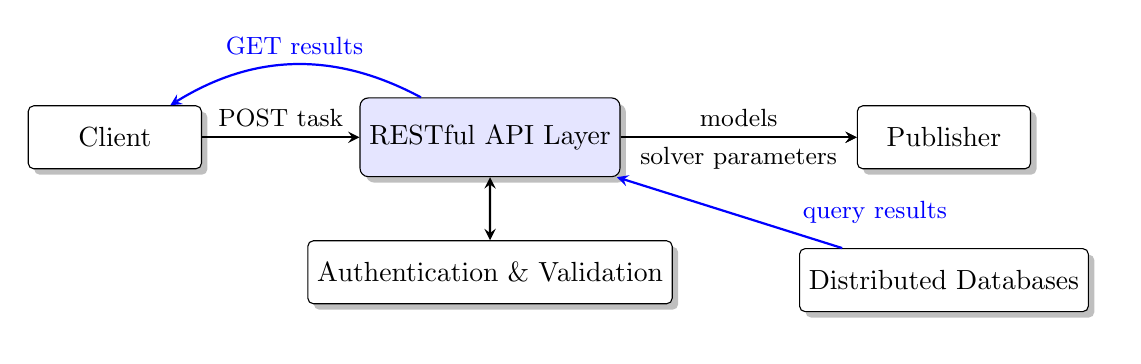
\begin{tikzpicture}[
      scale=0.8,
      >=stealth,
      box/.style={draw,rectangle,rounded corners=2pt,minimum width=2.2cm,
                  minimum height=0.8cm,align=center,fill=white,drop shadow},
      apibox/.style={draw,rectangle,rounded corners=3pt,minimum width=2.8cm,
                  minimum height=1cm,align=center,fill=blue!10,drop shadow},
      msg/.style={->, thick},
      label/.style={font=\small,draw=none}
    ]
    
    % Client
    \node[box] (client) {Client};
    
    % REST API Layer with its components
    \node[apibox, right=2cm of client] (api) {RESTful API Layer};
    \node[box, below=0.8cm of api] (auth) {Authentication \& Validation};
    
    % Publisher
    \node[box, right=3cm of api] (publisher) {Publisher};
    
    % Database
    \node[box, below=1cm of publisher] (db) {Distributed Databases};
    
    % Fit node for Backend System
    \node[fit=(api)(auth)(publisher)(db),
          draw, inner sep=0.3cm, dashed, 
          label={[yshift=0.3cm]\textbf{Backend System}}] (platform) {};
    
    % Draw connections
    \draw[msg] (client) -- node[above,label]{POST task} (api);
    \draw[msg] (api) -- node[above,label]{models} (publisher);
    \draw[msg] (api) -- node[below,label]{solver parameters} (publisher);

    % Two-way arrow between API and Auth
    \draw[<->, thick] (api) -- (auth);
    
    % Status monitoring path
    \draw[msg, blue] (api) to[bend right=30] node[above,label] {GET results} (client);
    
    % Database connections
    \draw[msg, blue] (db) -- node[right,xshift=0.8cm,label]{query results} (api);
    
  \end{tikzpicture}
  \caption{Simplified RESTful API architecture for the microservice.}
  \label{fig:rest-api-architecture}
\end{figure}

\section{Interoperability and Extensibility}
Through its API endpoints, the system exposes multiple established PRA solvers and provides a comprehensive list of quantification services. These services include probability calculation, cut set enumeration, common cause failure analysis, importance measures, safety integrity level assessment, and uncertainty quantification. To support these services, the architecture integrates multiple algorithmic engines and approximation methods, allowing the user to select the optimal computational path for their tasks based on model characteristics and performance requirements. Figure~\ref{fig:pracciolini} lists the tools supported by the interoperability layer and the model formats each tool uses.

\begin{figure}[]
  \centering
  \includesvg[width=\textwidth]{4-design/plots/pracciolini.svg}
  \caption{Example of supported model transitions in the operability layer.}
  \label{fig:pracciolini}
\end{figure}

The system achieves interoperability through a solver independent job specification that captures the essential parameters for PRA quantification. It includes the model reference, the analysis type, and the required outputs. Figure~\ref{fig:interoperability} shows the fields of this specification. This schema is called the \emph{intermediate JSON format}. Users can upload models in a tool specific format and select any supported solver. When a conversion path exists, the system converts the model to the format required by the chosen tool through this intermediate format behind the scenes.

\begin{figure}[]
  \centering
  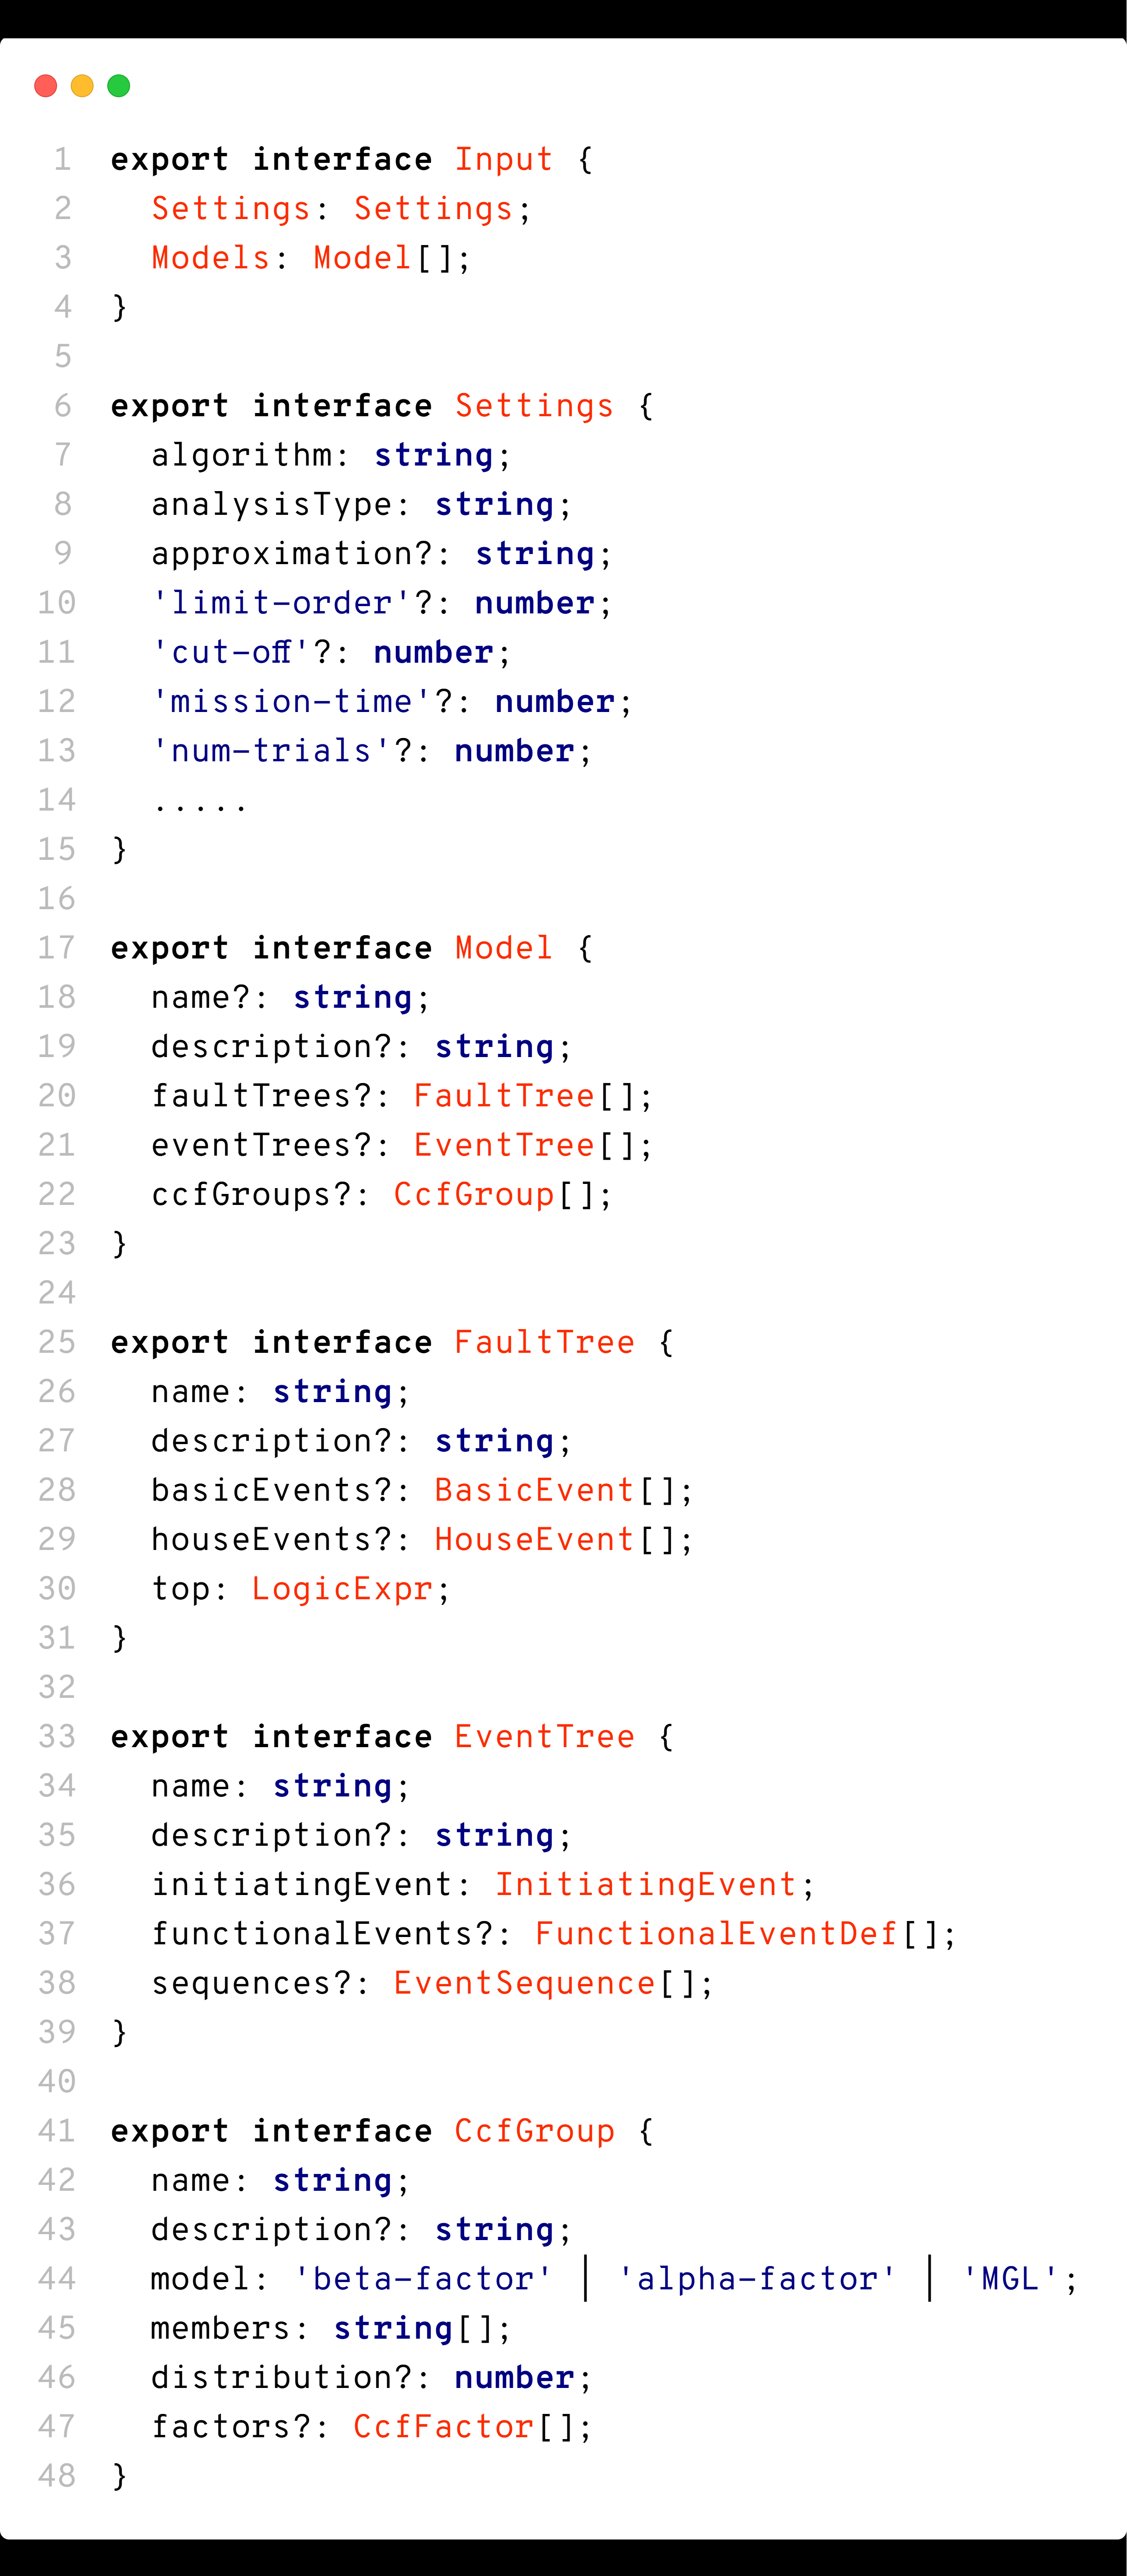
\includegraphics[width=0.60\linewidth]{4-design/plots/interoperability}
  \caption{Data structure of the intermediate JSON format.}
  \label{fig:interoperability}
\end{figure}

The architecture supports schema evolution through versioned interfaces, maintaining backward compatibility while enabling forward progress. All external interfaces are versioned, allowing the system to translate between different specification versions and ensuring existing workflows continue to function as the platform evolves to incorporate new computational approaches and data formats.

\section{Performance Optimization Strategies}
The system employs multiple queues to match workload characteristics, including first-in-first-out for fairness and priority queues for time sensitive computations. Work stealing improves resource utilization by allowing underutilized workers to claim tasks from overloaded queues.

Large models are parallelized differently depending on whether the analysis tool is closed source or open source. For closed-source tools, optimization of the internal algorithms is not feasible. Consequently, the only practical approach is to modify the input model. In this approach, an event tree can be dissociated into individual event sequences, after which each sequence is queued and quantified as a separate job. For open-source tools, more efficient code-level optimizations can be implemented. Rather than creating a separate representation for every dissociated input, a probabilistic directed acyclic graph (PDAG) is constructed only once for each event tree, and different parts of that PDAG are then distributed as separate jobs. This avoids repeatedly constructing equivalent PDAGs and significantly speeds up processing. In addition, the workflow uses adaptive quantification: an initial estimate of the sequence frequency is obtained using BDD based or Monte Carlo methods, and then cut sets are enumerated only up to a specified frequency truncation limit using internal algorithms. In this adaptive approach, cut sets are enumerated using ZBDD when following the BDD based path, and using MOCUS when following the Monte Carlo path.

This decomposition extends to importance measures, where basic event based analyses are queued separately, and uncertainty quantification, where each simulation run becomes an independent job. All results are aggregated deterministically using predefined output formats that specify the necessary data fields for reconstruction.

\section{Fault Tolerance Mechanisms}
The system ensures reliability through multiple approaches. Computational components employ a stateless design, allowing any worker to process tasks without storing any internal session data. As a result, the system can recover quickly by redirecting the jobs to healthy instances. Cascading failures are prevented by isolating degraded services and returning graceful error messages until these services recover.

Message processing guarantees at-least-once delivery, with idempotent operations ensuring duplicate messages are processed only once. Workers acknowledge messages only after successfully persisting results, while unacknowledged messages are automatically re-queued after configurable timeouts.

Health monitoring continuously checks components through regular ping intervals, triggering automatic remediation actions such as restarting failed containers to maintain system availability.

In addition, the system employs an exponential backoff reconnection strategy to handle message broker failures or restarts, retrying up to three times to reconnect. If reconnection is unsuccessful, the message is routed to the dead letter queue. Each message also includes a configurable time-to-live (TTL): if a worker cannot complete a quantification within the TTL window (default: 1 hour), the message expires and is moved to the dead letter queue to avoid saturating workers with stalled or long running tasks. Users may override the default TTL to control the maximum allowable processing time for their requests.

\section{Resource Management and Scalability}
The system’s resources are not auto scaled in response to workload. Instead, an administrator can scale the deployment up or down using the provided scripts: horizontally by adding or removing worker nodes in an on-premise cluster deployment, and vertically on a single node by increasing available resources through running multiple service instances across the node’s virtual CPUs (and GPUs where available).

A multi tenant resource model promotes fair usage through per-user quotas and queueing controls. Each user is subject to an individual request rate limit (default: 10 requests per hour) and a storage limit (default: 100 GB per user). The queueing system also supports priorities, but these priorities are not inferred automatically, jobs are ordered and processed according to the priority explicitly set by the user.

Hardware support depends on the deployment mode. Single node deployments can use both CPU and GPU capable workers, enabling GPU acceleration where applicable, while on-premise cluster deployments currently support CPU only workers. As a result, GPU execution is available only in the single node configuration, whereas cluster executions run entirely on CPU resources.

\section{Security and Access Control}
Authentication uses token based credentials validated with each request. Authorization follows the principle of least privilege through role based access control combined with attribute based policies. These policies grant access to proprietary tools only to licensed users, while unlicensed users are limited to open-source alternatives.

Multi tenancy ensures isolation between user environments, preventing unauthorized access to data or computational resources. Complete audit trails record all significant actions including model submissions and result accesses.

Data compression at client-server interfaces serves dual purposes: protecting sensitive nuclear facility data and compressing large input/output files to reduce storage usage.

\section{Operational Simplicity and Maintainability}
Operational simplicity is achieved through platform-as-code (PaaS) principles that enable reproducible deployments across all environments, supported by automated scaling for both planned expansion and emergency recovery.

Comprehensive monitoring is built into the architecture, with each component emitting standardized metrics, logs, and traces. The system tracks queue lengths, processing times, error rates, and resource utilization, providing real-time visibility into system health with automated alerting for anomalous conditions.

Detailed documentation covers API usage guidelines, deployment procedures, and implementation workflows through comprehensive markdown files and operational guides. The system also includes extensive test suites with both end-to-end integration tests and functional unit tests to verify system behavior.

\chapter{Implementation}

\section{PRA Solver Integration and Abstraction}
The first major challenge in developing a web-based ecosystem for PRA tools is tool integration. Integrating PRA tools is challenging because the supported tools differ in implementation language, invocation style, and input/output format. Some tools are closed source and available only as standalone executables, while others are open-source and can be customized as needed. To hide this complexity, the platform uses an adapter layer and a uniform asynchronous job based API. All requests are first validated against semantic schemas to reject malformed models and reduce the risk of script injection. After a request is accepted, the API immediately returns a job ID that can later be used to check job status or retrieve results. For decomposed event tree runs, the system may also return multiple job IDs associated with the event sequences.

For tools distributed as executables, both open-source and closed source solver binaries, together with their runtime dependencies, are packaged into the same container image as the worker service. This gives each worker direct local access to the solver. Users submit the model in the tool's native format, most commonly OpenPSA XML, but also tool specific formats such as JSInp for SAPHSOLVE, S2ML+SBE for XFTA, or .fta for FTREX, along with optional tool specific settings. If no settings are provided, default values are applied automatically. Because the worker services are written in TypeScript and accept JSON request bodies, raw model files are transmitted as base64 encoded strings. Base64 encoding allows file contents to be sent safely as printable text inside JSON. After receiving a request, the worker decodes the base64 data, writes it to a temporary file with a random name and the correct extension, constructs the same command line flags that the solver expects in normal CLI use, and invokes the executable through Node.js's child\_process.exec() method. The solver output is captured in a temporary result file, the contents of which are then to the object storage, and the temporary input and output files are then deleted.

For direct JSON based quantification, the platform currently supports SCRAM and PRAXIS \cite{praxis} without launching an external solver executable. SCRAM is written in C++, while PRAXIS is written in Rust and supports both CPU and GPU based Monte Carlo probability estimation. PRAXIS has been reproduced from a prior research work on data parallel Monte Carlo probability estimation \cite{arjun_2026}, because the original AGPL licensed implementation \cite{arjun_mcscram} could not be directly integrated into the MIT licensed distributed system as a solver. For both SCRAM and PRAXIS, native Node addons are written around the I/O, settings, and quantification classes/structs needed by the workers. A Node addon is ordinary C++ or Rust code compiled against the Node.js Addon API (Node API/N-API) \cite{napi}. Instead of producing an executable, the normal build system (e.g., CMake for C++ or Cargo for Rust) produces a \texttt{.node} shared library. This library can be imported directly into the TypeScript worker services. The addon exposes wrapper functions that map JSON fields to native C++ or Rust objects, call the underlying quantification routines, and map the native result objects back to JSON. In this way, the system keeps native code performance while still exposing a uniform TypeScript interface.

When users select SCRAM or PRAXIS, they submit the model in the OpenPRA JSON Model Exchange Format (MEF) \cite{openpra_documentation}, which was developed from the non-LWR technical elements standard ASME/ANS RA-S-1.4-2021 \cite{non_lwr_standard}. The model contains four main objects: \textbf{DA} - data analysis information, such as failure mode names, probabilities/frequencies, and distributions; \textbf{SA} - systems analysis information, including fault tree logic, \textbf{IE} - initiating event information, such as event names, grouping, and frequencies; and \textbf{ESA} - event sequence analysis information, including event tree logic, functional events, linked top events, failure/success/bypass states, and sequence names. Users also provide quantification settings, such as algorithm choice, requested analysis types, approximations, truncation limits, hardware selection etc. The request is routed to the appropriate worker function, which loads the required \texttt{.node} library, maps the JSON input to native data structures, executes the quantification, converts the native result structure back to JSON, and stores the result.

To execute native quantification reliably, the workers use a multi process design. Running a long native computation on the main Node.js thread would block the event loop and prevent the RabbitMQ connection from sending heartbeats. After a timeout, RabbitMQ may treat the worker as disconnected, drop the connection, and requeue the job. One possible solution is to offload the work to a separate thread, but that would require two threads per worker and leave the main thread largely idle. Instead, the parent process keeps the RabbitMQ connection alive, while a child process loads the addon and performs the quantification in its own memory space. This avoids dropped connections without wasting worker threads. Figure~\ref{fig:solver-integration} shows the internal architecture and workflow of each worker/consumer service.

\begin{figure}[]
  \centering
  \includesvg[width=1.10\textwidth]{5-implementation/plots/solver-integration.svg}
  \caption{Internal architecture and workflow of the worker/consumer services for PRA solver integration and result handling.}
  \label{fig:solver-integration}
\end{figure}

Event tree decomposition is supported in three ways, depending on the capabilities of the selected tool:
\begin{itemize}
    \item \textbf{Fault tree only tools (e.g., FTREX and XFTA):} The event tree is transformed into the logical OR of its individual event sequences. Each sequence is then converted into a fault tree and quantified independently. The final event tree result is obtained by OR-combining the sequence results.
    \item \textbf{Closed source tools with event tree support:} The original event tree input file is split into separate inputs, one per event sequence. Each sequence is quantified as an independent job, and the partial results are stitched back together afterward.
    \item \textbf{Open source tools with internal model access:} A lightweight addon first generates only the tool's internal PDAG representation for the full event tree. That PDAG is then partitioned by event sequence and the chunks are distributed to different workers. This avoids regenerating the PDAG for every sequence and reduces repeated preprocessing cost.
\end{itemize}

Result aggregation is also automated. Workers processing decomposed jobs use distributed coordination to determine when all related sequence jobs have finished. The final worker or coordinator then performs deterministic aggregation by extracting the required fields from the individual results according to predefined output schemas and stitching them into the final response. As a result, even when the system internally creates many sub-jobs, the user facing workflow remains simple: submit once, track the returned job ID(s), and retrieve the final result later.

\section{System Architecture Implementation}
\label{sec:sys-arch-implementation}
The deployed system combines three architectural styles: (i) a 4 tier client-server flow for non-quantification requests, (ii) a microservice based deployment where each component is packaged and scaled independently, and (iii) an event driven pipeline for long running quantification and tool execution jobs. From left to right, in Figure~\ref{fig:system-implementation}, the main components are the client, the reverse proxy, the API gateway (server backend), the message broker, the worker services, and the storage layer.

A client can be a web frontend, a lightweight library, or any code that can send HTTP(S) requests to the exposed API endpoints. Incoming requests first pass through a containerized reverse proxy:
\begin{itemize}
    \item \textbf{Traefik (multi node deployments):} used because it integrates well with on-premise cluster based deployments by providing dynamic routing and service discovery, built-in load balancing, and automated TLS certificate management.
    \item \textbf{Nginx (single node deployments):} used as the primary load balancer and reverse proxy. When all services run on a single machine, a static upstream configuration is sufficient for distributing requests across API gateway replicas.
\end{itemize}

\begin{figure}[]
  \centering
  \includesvg[width=\textwidth]{5-implementation/plots/system-implementation.svg}
  \caption{System implementation architecture showing the deployed components and their associated technology stack.}
  \label{fig:system-implementation}
\end{figure}

The reverse proxy intercepts client requests, applies routing, TLS, load-balancing as needed, and forwards traffic to an instance of the API gateway. The API gateway is implemented in NestJS \cite{noauthor_documentation_nodate}, a Node.js \cite{Node} based framework and written in TypeScript \cite{starting}.
The gateway is not only an HTTP entry point but also the place where request routing and the core backend logic live:
\begin{itemize}
    \item \textbf{Routing logic:} inspects the request URL and request type (non-quantification vs. quantification or execution), and for quantification/execution requests also identifies which tool or workflow is requested.
    \item \textbf{Business logic:} handles control plane operations such as creating and updating job records, storing and returning job status and error information, and returning metadata required to locate inputs or outputs.
    \item \textbf{Producer:} for long running compute requests, the gateway forwards the request to an internal producer module (also implemented inside NestJS). The producer serializes the request body into a message buffer and publishes it to the message broker.
\end{itemize}
Table~\ref{tab:endpoints} lists the main API entry points, together with their HTTP methods and a short description. The API gateway, business logic, and producer logic are deployed together as a single containerized backend service. Communication follows two complementary patterns:
\begin{itemize}
    \item \textbf{Synchronous HTTP APIs:} Used for non-quantification operations and job control, for example: submit a job and receive an acknowledgement, query job status, and retrieve stored results once available).
    \item \textbf{Asynchronous messaging (event driven):} Used for quantification and execution jobs that may take substantial time. These jobs are queued and processed by workers in the background.
\end{itemize}

\begin{landscape}
\begin{longtable}{@{}lll@{}}
\caption{Main entrypoints exposed by the API gateway.}
\label{tab:endpoints}\\
\toprule
\textbf{Endpoint} & \textbf{Methods} & \textbf{Description} \\
\midrule
\endfirsthead
\caption*{Table \thetable{} (continued).}\\
\toprule
\textbf{Endpoint} & \textbf{Methods} & \textbf{Description} \\
\midrule
\endhead
\bottomrule
\endfoot
%
\multicolumn{3}{@{}l}{\textbf{Executable Solver Submission}}\\
\midrule
\texttt{/q/execute/scram} & POST & Submit an executable based SCRAM quantification job \\
\texttt{/q/execute/ftrex} & POST & Submit an FTREX executable quantification job \\
\texttt{/q/execute/xfta} & POST & Submit an XFTA executable quantification job \\
\texttt{/q/execute/saphsolve} & POST & Submit a SAPHSOLVE executable quantification job \\
\texttt{/q/execute/<tool>?distributedSequences=true} & POST & Submit an executable task using event tree decomposition \\
\addlinespace
\multicolumn{3}{@{}l}{\textbf{Direct JSON Quantification}}\\
\midrule
\texttt{/q/quantify/scram} & POST & Submit a direct JSON based SCRAM quantification job \\
\texttt{/q/quantify/praxis} & POST & Submit a direct JSON based PRAXIS quantification job \\
\texttt{/q/quantify/<tool>?distributedSequences=true} & POST & Submit a quantification job using event tree decomposition \\
\addlinespace
\multicolumn{3}{@{}l}{\textbf{Job Retrieval and Monitoring}}\\
\midrule
\texttt{/execute/results/\{job\_id\}} & GET & Retrieve results for an executable based job \\
\texttt{/quantify/results/\{job\_id\}} & GET & Retrieve results for a direct quantification job \\
\texttt{/execute/status/\{job\_id\}} & GET & Retrieve status for an executable based job \\
\texttt{/quantify/status/\{job\_id\}} & GET & Retrieve status for a direct quantification job \\
\texttt{/execute/input/\{job\_id\}} & GET & Retrieve the submitted input for an executable based job \\
\texttt{/quantify/input/\{job\_id\}} & GET & Retrieve the submitted input for a direct quantification job \\
\end{longtable}
\end{landscape}

Asynchronous processing is implemented using RabbitMQ \cite{RabbitMQ}, an AMQP based message broker \cite{enwiki:1297038479}. RabbitMQ was selected because it provides reliable delivery with acknowledgements, flexible routing via exchanges  keys, durable queues, and operational features such as dead lettering and queue policies.

The producer publishes each job to one of two main queue classes: (i) quantification queue(s) and (ii) executable queue(s). In practice, each class may contain multiple (possibly temporary) queues, and RabbitMQ routes messages to the correct queue using the exchange routing key, i.e., the key indicates which queue family a message belongs to.

Queues are configured to be durable and messages are published as persistent. This ensures that both the queue definitions and the messages survive broker restarts and crashes, because RabbitMQ writes the relevant data to disk instead of memory. In addition, queue policies such as maximum queue length and message TTL are used. If a queue overflows or a message stays unprocessed for too long, it is moved to a dead letter queue instead of being endlessly re-queued, which would otherwise allow a stuck job to starve other jobs. RabbitMQ itself is deployed as a containerized service.

Compute is performed by separate worker services. Each worker service is a containerized NestJS application that runs RabbitMQ consumers. These worker services are kept separate from the API gateway. When a consumer is free and a message is available, it: (i) consumes the message, (ii) parses its contents to identify the job type and (iii) invokes the corresponding worker function.

Two execution paths, i.e., two types of worker functions are supported:
\begin{itemize}
    \item \textbf{Quantification jobs:} The worker passes the received JSON payload to a Node.js wrapper (Node addon). The addon maps the JSON data into native representations (C++ classes or Rust structs), executes the PRA quantification in the native codebase, and then converts the resulting objects back into JSON for storage.
    
    \item \textbf{Executable jobs:} The request payload contains the model encoded in Base64 format. The worker decodes it, converts it into the solver specific input format (e.g., OpenPSA for most solvers and JSInp for SAPHSOLVE), writes the model to corresponding temporary input file(s), and invokes the solver via a child process with the required command line flags and the directory of the temporary input file(s). The solver generates output files, which are read back by the worker and prepared for storage.
\end{itemize}

Workers are containerized together with the required solver executables and their dependencies. They are deployed as separate services so they can be scaled independently. For example, quantification workers can be scaled separately from executable workers.

Two non relational storage systems are used to match different access patterns:
\begin{itemize}
    \item \textbf{MongoDB \cite{MongoDB}:} Stores structured metadata such as job identifiers, submission parameters, timestamps, and run status/progress information.
    \item \textbf{MinIO \cite{minio}:} Stores large artifacts such as uploaded input files and generated output reports. MinIO provides a web interface that can be used to browse and download stored objects.
\end{itemize}
Both MongoDB and MinIO are deployed as containerized services and can be scaled separately from the compute layer. All major components: reverse proxy, API gateway, RabbitMQ, worker services, and storage services are packaged as Docker containers \cite{docker}. The system supports two deployment modes:

\begin{itemize}
    \item \textbf{Single node deployment:} all containers run on a single machine using standard Docker networking. In this mode, Nginx is used as the reverse proxy because the setup is static and no cross node service discovery is required.

    \item \textbf{On-premise multi node deployment using Docker Stack / Swarm:} the system is deployed as a Docker Stack, allowing services (API gateway replicas, worker replicas, RabbitMQ, and storage services) to be scheduled across multiple nodes. In this mode, overlay networks are used so that containers running on different machines can communicate as if they were on the same logical network. Overlay networking also enables clean network segmentation (e.g., restricting internal service-to-service traffic to the overlay network while exposing only the reverse proxy externally). Traefik is used in this mode because it can automatically discover services and apply routing and load-balancing rules dynamically as services scale up or down.
\end{itemize}

Overall, this containerized and modular design keeps services loosely coupled and independently scalable: the reverse proxy, backend, broker, worker pools, and storage can be scaled or updated without requiring the whole system to be redeployed.

\section{Scalability and Resource Management Implementation}
The system uses a manually deployed container based architecture defined through YAML files. Deployment begins by creating a Docker network. A single reverse proxy is then deployed to listen for incoming requests on ports 43 and 8080. After that, the core services are started in sequence: one RabbitMQ instance for job brokering, followed by MongoDB and MinIO. RabbitMQ currently runs as a single instance, whereas MongoDB and MinIO are deployed with multiple instances across multiple nodes. The worker tier is deployed next. At present, the system runs 128 workers, and each worker has direct access to the required solvers. Finally, multiple producer instances are deployed, and the reverse proxy load balances requests across them to maintain high throughput.

On the compute side, scalability is achieved by running many producers and workers in parallel rather than through fully automatic orchestration. Resource management focuses on assigning jobs to suitable hardware and preventing individual analyses from exhausting shared capacity. Workers can be deployed on specialized nodes, such as high memory nodes for ZBDD operations and standard CPU nodes for routine quantification. Resource limits are used to prevent memory intensive jobs from overwhelming a node. At present, GPU enabled executions are available only for single node based deployments and are not yet supported in on-premise cluster deployments.

Job scheduling also includes a priority and fair share mechanism. Each job can be assigned a priority level from 1 to 5, and each user is limited to a total of 50 priority points within a one hour window. This prevents any single user from monopolizing the system while still allowing urgent jobs to be submitted with higher priority.

Storage scalability is provided by MinIO in distributed mode and by MongoDB sharded clusters with hashed sharding keys, which distribute metadata evenly across replica sets. Together, these components allow the platform to support concurrent submissions, distribute quantification workloads across many workers, and store large result sets efficiently.

\section{Security and Access Control Implementation}
Security is implemented through JWT based authentication and role based access control. The API Gateway validates JWT tokens for every request, extracting user roles and permissions that determine access to specific solvers, models, and analytical services. Access to jobs and results is controlled through the same authentication and role based authorization, and ownership checks, which prevent unauthorized cross access to stored data.

All PRA models and results are encrypted using AES 256 encryption by default in MinIO object storage. The system encrypts sensitive nuclear facility data before storage and applies Brotli \cite{brotli} compression to reduce bandwidth.

Audit logging captures every significant action: model submissions, job executions, and result accesses with immutable timestamps and user identifiers. Logs are stored in a secure format for compliance and monitoring. Session management enforces automatic timeout after 30 minutes of inactivity, requiring re-authentication for continued access.

\section{Operational Monitoring, Testing, and Documentation}
The testing suite consists of Jest for unit tests and Supertest for API integration testing. Unit tests cover individual adapter functions and schema validators, while end-to-end tests verify full quantification pipelines, from job submission through result retrieval, using reference PRA models with known expected results.

Monitoring is implemented through Prometheus metrics that track number of queued jobs, worker utilization, error rates, and job completion times. Grafana dashboards provide real-time visibility into system health. Alert rules trigger notifications when critical thresholds are exceeded, such as increased queue backlogs or job failure rates.

Maintenance includes automated cleanup of temporary storage files. Health checks validate service availability every 30 seconds, with failed containers automatically restarted by Docker. Troubleshooting documentation provides step-by-step guidance for common failure scenarios, including solver specific error codes and recovery procedures.

All system components include comprehensive logging using structured JSON format, with unique IDs tracing requests across service boundaries. Log aggregation through the ELK stack enables efficient debugging and operational analysis.

Documentation forms an integral part of the implementation, with comprehensive guides covering system architecture, API references, deployment procedures, and operational practices. 

%Fig. \ref{fig:swagger_doc} shows the interactive API documentation generated by Swagger for the distributed system microservice, detailing its available endpoints, supported request methods, and operational descriptions.
%\begin{landscape}
\begin{figure}
    \centering
    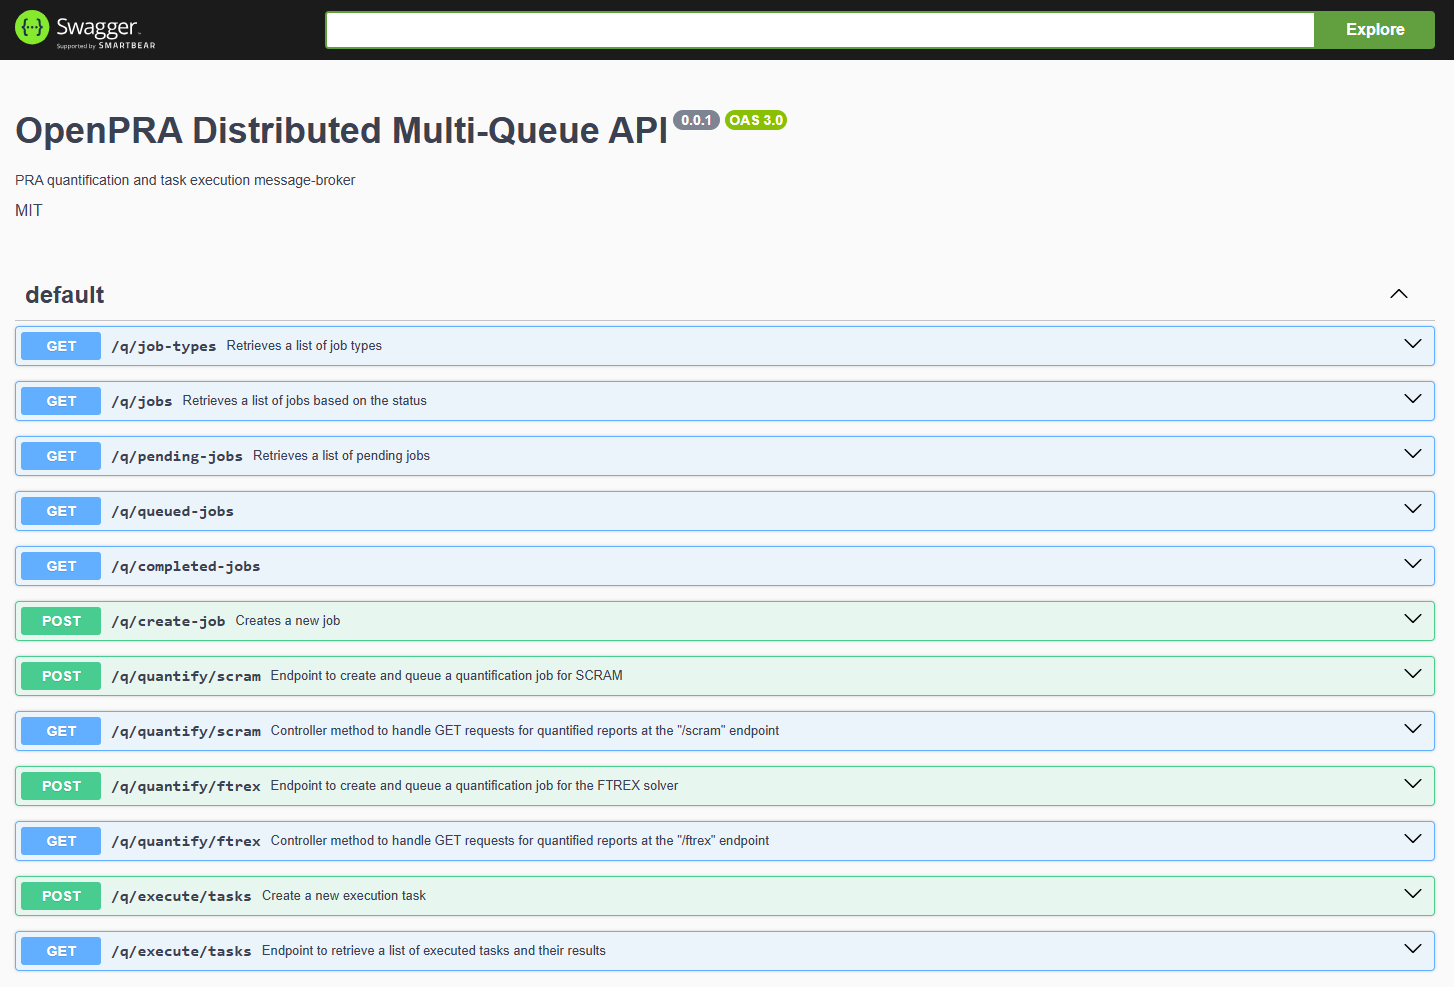
\includegraphics[width=1.3\textwidth]{5-implementation/plots/swagger_doc.png}
    \caption{Interactive API documentation detailing the endpoints available in the distributed networked system.}
    \label{fig:swagger_doc}
\end{figure}
\end{landscape}
\chapter{Case Study}
\label{chap:experiments}

\section{Model Description}

For the case study, a Probabilistic Risk Assessment (PRA) model for the Generic Modular High Temperature Gas Cooled Reactor (MHTGR) is used \cite{hamza_openpra-orggeneric-mhtgr-model_2025}, which was developed using SAPHIRE and CAFTA. The MHTGR plant comprises four identical 350 MW(t) reactor modules driving two shared turbine generators for a total output of approximately 558 MW(e).

The PRA model encompasses a comprehensive set of event trees and fault trees designed to capture the plant's response to initiating events. The analysis develops seven event trees, each based on a primary initiating event. Table~\ref{tab:mhtgr-initiating-events} shows the corresponding frequencies of the initiating events.

\begin{table}[]
\centering
\caption{MHTGR initiating events and frequencies}
\label{tab:mhtgr-initiating-events}
\begin{tabularx}{\textwidth}{l >{\RaggedRight}X r}
\toprule
\textbf{Initiating Event} & \textbf{Description} & \textbf{Frequency (per year)} \\
\midrule
PCL & Primary coolant leaks & $2.6 \times 10^{-1}$ \\
LOHTL & Loss of main loop cooling & $2.6 \times 10^{0}$ \\
LOOP & Loss of offsite power & $5.0 \times 10^{-3}$ \\
ATRS & Anticipated transients requiring SCRAM & $2.5 \times 10^{1}$ \\
CRW & Control rod withdrawal & $1.0 \times 10^{-1}$ \\
SGTL-S & Small steam generator leaks & $4.0 \times 10^{-1}$ \\
SGTL-M & Moderate steam generator leaks & $4.0 \times 10^{-2}$ \\
\bottomrule
\end{tabularx}
\end{table}

The event tree analysis models accident progression through safety functions including reactor shutdown, decay heat removal, and containment isolation. The complete model comprises 241 event sequences distributed across these 7 event trees as shown in Table~\ref{tab:mhtgr-event-tree-sequences}.

\begin{table}[]
\centering
\caption{Event tree sequences in the MHTGR PRA model}
\label{tab:mhtgr-event-tree-sequences}
\begin{tabularx}{\textwidth}{l >{\RaggedRight}X r}
\toprule
\textbf{Initiating Event} & \textbf{Key Safety Functions} & \textbf{Sequences} \\
\midrule
Small SG tube leaks (SGTL-S) & Moisture detection, SG isolation, decay heat removal & 1 to 46 (46) \\
Primary coolant leaks (PCL) & Reactor trip, RSCE shutdown, SCS/RCCS cooling & 47 to 96 (50) \\
Anticipated transients (ATRS) & SCRAM logic, backup shutdown, heat removal & 97 to 130 (34) \\
Control rod withdrawal (CRW) & PPIS detection, reactor trip, power excursion control & 131 to 138 (8) \\
Loss of offsite power (LOOP) & Reactor trip, backup power, passive cooling & 139 to 150 (12) \\
Moderate SG tube leaks (SGTL-M) & Rapid isolation, pressure control, backup cooling & 151 to 213 (63) \\
Loss of HTS cooling (LOHTL) & Forced convection loss, shutdown, emergency cooling & 214 to 241 (28) \\
\midrule
\textbf{Total} & & \textbf{241} \\
\bottomrule
\end{tabularx}
\end{table}

The fault tree analysis provides detailed reliability models for critical safety systems, with each tree typically decomposed into 5 to 15 subsystems. The primary systems modeled are listed in Table~\ref{tab:fault-tree-systems}.

\begin{table}[]
\centering
\caption{Fault tree models for MHTGR safety systems}
\label{tab:fault-tree-systems}
\begin{tabularx}{\textwidth}{l >{\RaggedRight\arraybackslash}X}
\toprule
\textbf{System} & \textbf{Safety Function} \\
\midrule
Heat transport system (HTS) & Primary heat removal via forced helium circulation \\
Shutdown cooling system (SCS) & Active decay heat removal using auxiliary blower loop \\
Reactor cavity cooling system (RCCS) & Passive heat removal from reactor vessel \\
Reserve shutdown control (RSCE) & Backup neutron absorbing material injection \\
Steam isolation and dump system & Secondary system isolation and pressure control \\
Relief valves & Primary and secondary system pressure relief \\
Reactor trip system & Control rod scram and reactor shutdown \\
%Failure to trip reactor using RSCE (FT34)
%Failure of HTS in at least One Module (FT104)
%Failure of SCS When One Module Requires Cooling (FT174)
%Failure of SCS (FT196)
%Failure of SCS when Four Modules Require Cooling (FT197, FT198 and FT199)
%Intentional depressurization fails (FT215)
\bottomrule
\end{tabularx}
\end{table}

The model includes 170 basic events representing distinct component failure modes and approximately 100 repair events to account for system recovery processes. These events are parameterized with mean failure frequencies or probabilities based on component type and operational context.

\section{Setup Description}
The study used four solver configurations: SAPHSOLVE (Windows version), serial SCRAM, distributed SCRAM, and PRAXIS (in both CPU and GPU modes). All solver configurations were set to compute event sequence frequencies and the number of minimal cut sets for each event sequence. Three truncation settings were evaluated: no truncation, to determine whether all cut sets could be captured, and truncation limits of $10^{-12}$ and $10^{-20}$. Single machine CPU based executions were performed on a system with an Intel i7-13700K processor and 32~GB of RAM under standard processing conditions. Single machine based PRAXIS GPU runs were executed on a workstation equipped with an NVIDIA RTX PRO 6000 Blackwell Max-Q Workstation Edition GPU with 96~GB of GDDR7 memory. Distributed quantifications were executed on a high performance on premise cluster with 12 nodes. For this study, only 5 nodes were used: 1 manager node and 4 worker nodes. The manager and worker nodes are equipped with Intel Xeon CPUs (24 and 128 vCPUs, respectively), 128~GB and 256~GB of RAM, and 4~TB and 1~TB of NVMe storage, respectively. The deployment was scaled to support up to 128 workers.

\subsection{Description of the Studies}
Four studies were performed to evaluate the proposed distributed quantification system. Together, they demonstrate the capabilities and advantages of the system, highlight its limitations, and examine the effectiveness of the measures introduced to mitigate those limitations.

(a) \textbf{Multiple concurrent job handling:}
The first study evaluates how well the distributed system handles large numbers of concurrent jobs submitted by users. It focuses on scalability and speedup as the number of workers increases. The CRW event tree is quantified using three configurations: SAPHSOLVE (serial), SCRAM (serial), and distributed SCRAM. For distributed SCRAM, the number of workers is varied from $2$ to $128$, while the number of simultaneously submitted jobs is varied from $1$ to $10,000$.

(b) \textbf{Robust execution of large event tree jobs:}
Very large quantification tasks can run for a long time, become stuck, or fail after many hours, making it difficult to determine whether they will ever complete and risking complete loss of computational effort upon failure. The second study addresses this by introducing a three stage workflow (preprocessing, processing, and postprocessing) in which a large event tree is decomposed into individual event sequences. This decomposition enables partial retention of results, even if some sequences fail, and allows the distributed system to requeue failed jobs or to move repeatedly failing jobs into dead letter queues, and to continue processing the remaining sequences. In this way, the system aims to guarantee execution of large event tree jobs in a fault tolerant manner, or at least to preserve partial results under worker or job failures. For this study, the MHTGR model is quantified using SAPHSOLVE, serial and distributed SCRAM with $2$ to $128$ workers.

(c) \textbf{Stress testing:}
The final study focuses on the overall throughput and latency of the distributed system under large request loads. The LOOP event tree is used with a truncation limit of $10^{-12}$. This model is repeatedly submitted to the quantification API endpoint up to $10^{6}$ times, and an equal number of requests is then issued to retrieve the corresponding results. The number of workers is fixed at $128$ for this stress test. The objective is to determine how many quantification requests and result-retrieval operations the system can handle concurrently without failure, and to characterize the limits at which throughput and latency begin to degrade, even for relatively small jobs with a large worker pool.

The next section presents the detailed description and the results of these four studies.

\section{Results and Discussion}
\subsection{Concurrent Job Handling and Performance}
This study evaluates how well distributed SCRAM handles large numbers of concurrent jobs and how its performance changes as the workload increases. Practical PRA studies can contain tens of event trees, tens to hundreds of fault trees, and hundreds of event sequences. Repeated calculations of this kind also appear in sensitivity, importance, and uncertainty analyses, where the same quantification must be performed many times while only the probabilities of basic events or CCF groups are changed.

The CRW event tree from the MHTGR model was used as the benchmark model. One full evaluation of the CRW event tree was counted as one job. Since the CRW event tree contains 8 event sequences, the workload range of 1 to 10{,}000 jobs corresponds to 8 to $8.00E+04$ event sequences in total. A comparison is made between serial SAPHSOLVE (Windows version), single-process SCRAM, and distributed SCRAM configurations using 2, 4, 8, 16, 32, 64, and 128 workers. As a representative example, 10{,}000 jobs correspond to changing the probabilities of 1{,}000 basic events from 0.1 to 1.0 in increments of 0.1.

\begin{figure}[htbp]
  \centering
  \includesvg[width=1\textwidth]{6-experimental-evaluation/figures/performance.svg}
  \caption{Execution time of as a function of the number of submitted jobs (from $1$ to $1000$) for SAPHSOLVE, SCRAM, and distributed SCRAM with 2 to 128 workers.}
  \label{fig:performance}
\end{figure}
\begin{figure}[htbp]
  \centering
  \includesvg[width=1\textwidth]{6-experimental-evaluation/figures/speedup.svg}
  \caption{Speedup relative to SCRAM Serial as a function of the number of concurrent jobs (from $1$ to $10000$) for SAPHSOLVE, SCRAM, and distributed SCRAM with 2 to 128 workers.}
  \label{fig:speedup}
\end{figure}

Figure~\ref{fig:multiple_concurrent_job} shows the wall-clock time as a function of the number of jobs and workers, and figure~\ref{fig:performance} shows the speedup of the distributed system relative to the serial solvers for different numbers of workers. At the low end of the workload range, the fixed cost of job creation, queueing, broker communication, dispatch, worker coordination, and result collection dominates. For this reason, when only a few jobs are submitted, single process SCRAM is usually faster than the distributed configurations, and increasing the number of workers beyond the number of available jobs provides little benefit. As the number of jobs increases, this fixed overhead is amortized, the workers remain busy for longer periods, and the benefit of distributed execution becomes clear.

For $1{,}000$ jobs, SAPHSOLVE required about $9.31E+03$~seconds ($\approx 1.55E+02$~minutes), while single process SCRAM required about $6.57E+03$~seconds. Distributed SCRAM reduced the runtime to about $3.53E+03$, $1.99E+03$, $8.53E+02$, $4.29E+02$, $2.16E+02$, $1.15E+02$, and $6.60E+01$~seconds for 2, 4, 8, 16, 32, 64, and 128 workers, respectively. For $10{,}000$ jobs, SAPHSOLVE required about $9.31E+04$~seconds ($\approx 2.59E+01$~hours), while single process SCRAM required $6.56E+04$~seconds ($\approx 1.82E+01$~hours).

The speedup $S(N)$ for $N$ workers is defined in the standard way as:
\begin{equation}
  S(N) = \frac{T_{\text{serial}}}{T_{\text{parallel}}(N)}
\end{equation}
where $T_{\text{serial}}$ is the wall-clock time of the single process SCRAM run, and $T_{\text{parallel}}(N)$ is the wall-clock time when the same workload is executed using $N$ workers in the distributed system. Using distributed SCRAM, the wall-clock time was reduced to approximately $3.43E+04$, $1.70E+04$, $8.53E+03$, $4.29E+03$, $2.17E+03$, $1.14E+03$, and $6.45E+02$~seconds for 2, 4, 8, 16, 32, 64, and 128 workers, respectively. Taking the single process SCRAM runtime as the serial baseline for the $10{,}000$ job case, the corresponding speedups are 1.91x, 3.85x, 7.69x, 15.30x, 30.16x, 57.52x, and 101.67x.

Even though the jobs in this experiment are independent and, in principle, $100\%$ parallelizable, the scaling curves still show behavior similar to Amdahl's law. The computational part of each job is embarrassingly parallel, but the full workflow still contains serial and overhead components that do not disappear when more workers are added. Jobs must be created by the producer, submitted to the message broker, placed in a queue, dispatched to workers, and collected again when the results are returned. Each worker must receive a job, deserialize its input, initialize or load the model if necessary, execute the analysis, serialize the results, and send them back. These additional steps introduce time that cannot be parallelized.

As the number of jobs increases, the system initially shows near linear scaling, but the speedup eventually begins to flatten. For a fixed number of workers, increasing the number of jobs increases queueing delay (latency) because more jobs must wait before a worker becomes available. For a fixed workload, adding more workers reduces the computation time per worker, but it does not remove the above mentioned overheads. As a result, these costs become a larger fraction of the total runtime at high worker counts.

This explains why, even with 128 workers, the maximum observed speedup for $10{,}000$ jobs is 101.67x rather than the ideal 128.00x. The gap can be attributed to the time required for the producer to package and enqueue each job, network latency between the producer, the message broker, and the workers, internal routing delay inside the message broker, the cost of serializing and deserializing job data, worker side model initialization, and contention for shared resources such as disks or file systems when writing logs or saving results.

An important feature of this study is that the resulting cut sets remain the same and only the overall probabilities or frequencies change. Because of this, the runtime of each job is very similar. This symmetric workload is easy to balance across workers and contributes to the good, though not perfectly linear, scaling observed in the figures. Overall, the results show that distributed SCRAM can substantially reduce the execution time of large batches of independent PRA calculations, including sensitivity analyses, importance measure studies, uncertainty quantification, and repeated scenario evaluations, while also showing that communication and coordination overhead place a practical upper bound on the achievable speedup.

\subsection{Robust Execution of Large Event Tree Jobs}
Very large event tree quantification jobs are difficult to execute robustly because a single stalled or failed run can waste many hours of computation and provide little information about which part of the model caused the problem. To study this behavior, the full set of MHTGR event trees was quantified at a truncation limit of $1E-20$ using SAPHSOLVE and SCRAM. In the baseline run, each event tree was submitted as a single large job without event sequence decomposition. Under this setup, both tools were able to solve only 5 of the 7 event trees. In particular, the PCL and ATRS event trees could not be solved. The baseline results have been summarized in Table~\ref{tab:mhtgr_robust_run1}.

\begin{table}[]
\centering
\caption{Baseline event tree level quantification results for the seven MHTGR event trees at a truncation limit of $10^{-20}$.}
\label{tab:mhtgr_robust_run1}
\small
\begin{tabular}{@{}lrrr@{}}
\toprule
\textbf{Event tree} & \textbf{Minimal cut sets} & \textbf{SAPHSOLVE (s)} & \textbf{SCRAM (s)} \\
\midrule
SGTL-S & $1.75 \times 10^{5}$ & $1.37 \times 10^{1}$ & $3.75 \times 10^{1}$ \\
PCL & N/A & N/A & N/A \\
ATRS & N/A & N/A & N/A \\
CRW & $3.25 \times 10^{6}$ & $1.76 \times 10^{2}$ & $9.24 \times 10^{1}$ \\
LOOP & $4.34 \times 10^{4}$ & $4.02 \times 10^{0}$ & $5.81 \times 10^{1}$ \\
SGTL-M & $2.33 \times 10^{5}$ & $2.02 \times 10^{1}$ & $5.42 \times 10^{1}$ \\
LOHTL & $5.36 \times 10^{6}$ & $2.53 \times 10^{2}$ & $4.21 \times 10^{2}$ \\
\bottomrule
\end{tabular}
\end{table}

The same calculation was then repeated in the distributed system using the SAPHSOLVE and SCRAM executables via the \texttt{/q/execute/saphsolve} and \texttt{/q/execute/scram} endpoints, with event sequence decomposition enabled. For SAPHSOLVE, this was done by splitting the input file into separate event sequence inputs, since SAPHSOLVE is closed source and only its file level interface can be manipulated. For SCRAM, the PDAG construction step was decomposed. In the original executable workflow, individual PDAGs are created and quantified in a "for" loop. In the distributed workflow, the PDAGs for all event sequences are obtained first and then distributed to workers, which quantify them independently and return sequence level results for final aggregation. The results of this second run have been summarized in Table~\ref{tab:mhtgr_robust_run2}.

\begin{table}[]
\centering
\caption{Sequence decomposed execution results for the seven MHTGR event trees at a truncation limit of $10^{-20}$.}
\label{tab:mhtgr_robust_run2}
\small
\begin{tabular}{@{}lrrr@{}}
\toprule
\textbf{Event tree} & \textbf{Minimal cut sets} & \textbf{SAPHSOLVE (s)} & \textbf{SCRAM (s)} \\
\midrule
SGTL-S & $1.75 \times 10^{5}$ & $1.55 \times 10^{1}$ & $3.75 \times 10^{1}$ \\
PCL & $8.30 \times 10^{8}$ & $1.51 \times 10^{5}$ & $1.90 \times 10^{4}$ \\
ATRS & $2.10 \times 10^{8}$ & $2.46 \times 10^{4}$ & $1.89 \times 10^{3}$ \\
CRW & $3.25 \times 10^{6}$ & $2.18 \times 10^{2}$ & $9.96 \times 10^{1}$ \\
LOOP & $4.34 \times 10^{4}$ & $4.28 \times 10^{0}$ & $5.83 \times 10^{1}$ \\
SGTL-M & $2.33 \times 10^{5}$ & $2.22 \times 10^{1}$ & $5.43 \times 10^{1}$ \\
LOHTL & $5.36 \times 10^{6}$ & $2.91 \times 10^{2}$ & $4.22 \times 10^{2}$ \\
\bottomrule
\end{tabular}
\end{table}

A direct comparison of the two result summaries shows the main trade-off of this approach. For event trees that were already solvable in the baseline run, sequence level decomposition adds a small amount of overhead because the system must split the work, dispatch more jobs, and aggregate the returned results. However, this overhead is outweighed by the gain in robustness for difficult jobs. In the decomposed workflow, SCRAM was able to quantify all event trees, including PCL and ATRS, which failed in the original run. For SAPHSOLVE, ATRS also became solvable, and the PCL failure no longer appeared as an unexplained full job failure. Instead, the problematic sequence was isolated to PCL-63.

This is the main advantage of the preprocessing, processing, and postprocessing workflow. Failed sequence jobs can be re-queued for quantification automatically, and if a sequence keeps failing it can be moved to a dead letter queue while the remaining event sequences continue to run. As a result, the full run does not lose all completed work, and the user still receives the partial results together with a clear indication of which sequence caused the problem. In this study, PCL-63 continued to fail in SAPHSOLVE and was therefore moved to the dead letter queue, while the remaining sequences completed normally.

In the decomposed run, the two dominant event trees were PCL and ATRS. PCL generated $8.30E+08$ minimal cut sets and required approximately $4.20E+01$~h in SAPHSOLVE and $5.28E+00$~h in SCRAM, while ATRS generated $2.10E+08$ minimal cut sets and required approximately $6.84E+00$~h in SAPHSOLVE and $5.25E-01$~h in SCRAM. At the event sequence level, the three largest contributors were PCL-91, PCL-76, and PCL-63, which generated approximately $3.67E+08$, $2.23E+08$, and $1.99E+08$ minimal cut sets, respectively. This explains why the PCL event tree dominates the total execution time and why sequence level distribution is especially useful for such workloads.

The main points of this calculation are summarized below:
\begin{itemize}
    \item Sequence level decomposition changed the previously unsolved PCL and ATRS event trees into solvable workloads in SCRAM.
    \item For SAPHSOLVE, decomposition exposed the main failure point as PCL-63 instead of losing the entire PCL job without diagnosis.
    \item The distributed workflow improved robustness by allowing successful sequences to finish, failed sequences to be retried, and repeatedly failing sequences to be moved to a dead letter queue.
    \item The approach also revealed the main computational hotspots, namely PCL-91, PCL-76, and PCL-63, which produced the largest numbers of minimal cut sets and dominated the runtime.
\end{itemize}

Overall, these results show that event sequence decomposition is not only a parallelization strategy but also a robustness mechanism. It makes large event tree jobs easier to diagnose, more fault tolerant during execution, and less likely to lose all computational effort when part of the workload fails.

\subsection{Load Testing / Stress Testing}

\begin{figure}[htbp]
  \centering
  \includesvg[width=1\textwidth]{6-experimental-evaluation/figures/load_test_analysis.svg}
  \caption{Performance analysis of microservices deployment showing (a) heavy batch processing scaling, (b) high concurrency limits, and (c) sustained load stability.}
  \label{fig:load_test_analysis}
\end{figure}

\subsubsection{Test 1: Heavy batch processing (LOOP Model)}
In this scenario, a workload consisting of 10,000 users submitting heavy batch jobs ($>0.5MB$), each requiring the decomposition of event trees into individual sequences, was simulated. As shown in \textbf{Figure 1(a)}, scaling the number of job brokers from 1 to 6 resulted in a linear increase in throughput (from $25.6$ to $132.5$ req/s) and a significant reduction in latency (from $2.52$s to $0.48$s). However, increasing the replicas to 8 caused a sharp degradation in performance, with throughput dropping to $38.9$ req/s. This indicates a bottleneck caused by connection instability rather than computation limits. Specifically, the intense traffic saturated the message queueing and object storage services (RabbitMQ and MinIO), preventing them from responding to health check pings; this triggered connection drops after two consecutive health check failures. Consequently, \textbf{6 brokers} was identified as the optimal configuration for such heavy workload.

\subsubsection{Test 2: High concurrency limits (Chinese Model)}
For lightweight, non-batch jobs ($\sim 3KB$), the system limits were evaluated by increasing the number of concurrent users from 10,000 to 25,000. \textbf{Figure 1(b)} illustrates that the system maintained a $0\%$ error rate up to 15,000 users. However, pushing beyond this threshold to 20,000 users introduced a $1.13\%$ error rate, despite the throughput remaining relatively stable. Furthermore, scaling brokers from 8 to 64 at the safe limit of 10,000 users yielded negligible gains, plateauing at $\sim1200$ req/s. This suggests that for lightweight jobs, the bottleneck again shifts downstream to the ingestion capacity of the message broker and object storage services (RabbitMQ/MinIO).

\subsubsection{Test 3: Sustained load stability}
To assess long-term stability, the system was subjected to a sustained load of 10,000 users for 10 minutes. \textbf{Figure 1(c)} demonstrates that the system remained highly stable across 8, 16, and 64 broker configurations, processing over 1.4 million requests without failure. While the 64-broker setup provided the lowest latency ($3.97$s) and highest throughput ($1212$ req/s), the 8-broker configuration was surprisingly competitive, recording $4.18$s latency and $1195$ req/s throughput. This reinforces the conclusion that for sustained, lightweight workloads over-provisioning brokers provides diminishing returns.

\begin{table}[htbp]
    \centering
    \caption{Summary of load testing results and bottleneck analysis}
    \label{tab:load-test-summary}
    \begin{tabular}{@{}llll@{}}
        \toprule
        \textbf{Test ID} & \textbf{Workload Type} & \textbf{Optimal Config} & \textbf{Primary Bottleneck} \\ 
        \midrule
        Test 1 & Heavy Batch ($>0.5$ MB) & 6 Brokers & Brokers and service connection timeouts \\
        Test 2 & High Concurrency ($\sim3$ KB) & 15,000 Users (Max) & Brokers and service connection limits \\
        Test 3 & Sustained Load (10 min) & 8 Brokers & N/A (diminishing returns) \\
        \bottomrule
    \end{tabular}
\end{table}

\subsection{Cost Estimate for Cloud Based Deployment}
\begin{figure}[H]
  \centering
  \includesvg[width=\textwidth]{6-experimental-evaluation/figures/aws.svg}
  \caption{High level overview of the AWS infrastructure deployment for PRA quantification purposes.}
  \label{fig:aws}
\end{figure}

To place the performance and cost profile of the distributed system presented in this work in perspective, the costs associated with running an identical workload on a state-of-the-art commercial cloud platform were analyzed. The projected operational expenditure for such an AWS hosted environment is estimated at approximately \$11,413 per month. The primary cost drivers are security governance (IAM Access Analyzer) and high volume storage (S3), which together account for over 55\% of the monthly budget. This estimate assumes a consistent workload utilizing 128 instances and significant message brokerage capacity to handle the load defined in the previous stress tests.

To derive these figures, usage patterns were modeled based on a user base of 10,000 active participants. The API Gateway costs were calculated assuming each user operates at the rate limit of 10 requests per hour continuously (24 hours over 30 days), resulting in a total of 72 million monthly requests. Identity management (IAM) costs reflect the maximum allowance of 10,000 distinct monitored accounts. Compute and messaging resources were provisioned to match the stress test environment, consisting of a single EKS cluster orchestration plane managing 128 EC2 worker nodes (1 vCPU, 4 GB RAM each) and 8 dedicated Amazon MQ broker instances. Storage costs for S3 are projected based on a hard cap of 10 GB per user, totaling 100 TB of persistent data.

It is important to note that several managed AWS services were explicitly excluded from this estimate as their functionality is handled by platform-agnostic alternatives in our architecture. Specifically, external container registries (Docker Hub/GitHub Container Registry) are used instead of Amazon ECS, dead letter queues (DLQs) are managed natively within RabbitMQ, autoscaling is handled through KEDA, and MongoDB is used in place of Amazon DynamoDB.

\begin{table}[htbp]
    \centering
    \caption{AWS Infrastructure Cost Estimate (US East - Ohio)}
    \label{tab:aws-cost-estimate}
    \begin{tabular}{@{}llrr@{}}
        \toprule
        \textbf{Service} & \textbf{Configuration Details} & \textbf{Monthly (USD)} & \textbf{Annual (USD)} \\ 
        \midrule
        IAM Access Analyzer & 10,000 accounts monitored & 4,000.00 & 48,000.00 \\
        S3 Standard & 100 TB storage, Data transfer & 2,321.74 & 27,860.88 \\
        Amazon EC2 & 128 $\times$ m6g.medium & 1,812.74 & 21,752.83 \\
        Amazon MQ & 8 $\times$ m5.large (RabbitMQ) & 1,784.32 & 21,411.84 \\
        Amazon CloudWatch & Metrics \& DB Insights & 1,168.90 & 14,026.80 \\
        Amazon API Gateway & 72M Requests/mo & 252.00 & 3,024.00 \\
        Amazon EKS & 1 Cluster & 73.00 & 876.00 \\
        \midrule
        \textbf{Total} & & \textbf{\$11,412.70} & \textbf{\$136,952.40} \\
        \bottomrule
    \end{tabular}
\end{table}
%\chapter{Discussion}
    \section{Analysis of Experimental Results}
    \section{Comparison with Existing PRA Tools}
    \section{Strengths and Limitations of the Proposed System}
    \section{Lessons Learned}
\chapter{Future Work and Conclusion}
\section{Future Directions}

The following enhancements are planned for the distributed PRA quantification system:

\begin{enumerate}
    \item Implement caching mechanisms for the adaptive method to store intermediate results at each truncation limit or limit order, preventing redundant calculations by reusing previously computed cut sets when increasing precision.

    \item Integrate the GPU accelerated Monte Carlo solver in the distributed system, extending the distributed framework to support heterogeneous computing environments with automatic resource allocation.

    \item Implement variance reduction techniques (importance sampling and stratified sampling) in the Monte Carlo + MOCUS adaptive quantification to tighten convergence for event sequences with frequencies below $10^{-9}$.

    \item Develop priority based queueing systems using directed acyclic graph algorithms to automatically assign task priorities based on computational complexity and available computational resources of the nodes.

    \item Implement Kubernetes based and Ansible controlled auto scaling features for dynamic resource provisioning, enabling automatic scaling of worker instances in response to workload demands.

    %\item Investigate and resolve RabbitMQ TCP connection issues while migrating from Minio to more robust storage solutions like Garage, which offers unrestricted usage and comprehensive logging capabilities.

    \item Transition from the current Platform-as-a-Service model to a Software-as-a-Service solution, hosting computational resources on dedicated on-premise clusters to eliminate infrastructure management related worries for the user.

    \item Expand solver integration by incorporating additional quantification algorithms, providing users with diverse methodological options for risk assessment.

    \item Extend benchmarking efforts to include importance measures and uncertainty quantification analyses, demonstrating system performance across the complete PRA calculation spectrum.
\end{enumerate}

\section{Closing Remarks}
This thesis has introduced a distributed computing framework for probabilistic risk assessment that addresses the computational limitations of traditional serial approaches. The literature review established the current landscape of PRA tools and identified critical gaps in distributed computing capabilities for nuclear risk analysis. Building upon distributed systems theory, the research presented a comprehensive architectural design that enables distributed processing of PRA quantification tasks.

The implemented system integrates existing PRA solvers within a scalable distributed environment, incorporating fault tolerance mechanisms. Through the MHTGR case study, the framework illustrated the scalability of the overall architecture when handling real world event trees and fault trees. The evaluation revealed both the system’s capabilities and limitations, particularly in adaptive quantification techniques, which informed the proposed future directions for enhancement, including integration of variance reduction techniques for the Monte Carlo fallback.

This work establishes a foundation for next generation PRA tools that can leverage distributed computing resources to handle increasingly complex risk models efficiently. The research contributions span theoretical framework development for adaptive quantification, practical system implementation with GPU accelerated Monte Carlo support, and code-to-code verification, providing a pathway toward more comprehensive and near real-time risk assessments in nuclear safety applications.


\printbibliography[
heading=bibintoc,
title={References}
]
%%\bibliography{bibliography}
%%\bibliographystyle{ieeetr}

\backmatter

\end{document}